\index{Clocks@\te{Clocks} (package)}


{\bf Package}

\begin{verbatim}
import Clocks :: * ;
\end{verbatim}


{\bf Description}

The BSV \te{Clocks} library provide features to access and change
the default clock.  Moreover, there are hardware primitives to
generate clocks of various shapes, plus several primitives which
allow the safe crossing of signals and data from one clock domain
to another.

The \te{Clocks} package uses the data types \te{Clock} and \te{Reset}
as well as clock functions which are described below but defined in the \te{Prelude} package.  

Each section describes a related group of modules, followed by a table
indicating the Verilog modules used to implement the {\BSV} modules.

{\bf Types and typeclasses}
\index{Clock@\te{Clock} (type)}
\label{package-clock}

The \te{Clocks} package uses the abstract data types \te{Clock} and \te{Reset},
which are defined in the \te{Prelude} package.  These are first class
objects.  Both \te{Clock} and
\te{Reset} are in the \te{Eq} type class, meaning two values can be
compared for equality.

\te{Clock}  is an abstract  type of two components: a single \te{Bit}
oscillator and a \te{Bool} gate.

\begin{libverbatim}
     typedef ... Clock ; 
\end{libverbatim}

\te{Reset} is an abstract type.
\index{Reset@\te{Reset} (type)}

\begin{libverbatim}
     typedef ... Reset ; 
\end{libverbatim}

\begin{center}
\begin{tabular}{|c|c|c|c|c|c|c|c|c|c|}
\hline
\multicolumn{10}{|c|}{Type Classes for \te{Clock} and \te{Reset}}\\
\hline
\hline
&\te{Bits}&\te{Eq}&\te{Literal}&\te{Arith}&\te{Ord}&\te{Bounded}&\te{Bitwise}&\te{Bit}&\te{Bit}\\
&&&&&&&&\te{Reduction}&\te{Extend}\\
\hline
\te{Clock}&&$\surd$&&&&&&&\\
\hline
\te{Reset}&&$\surd$&&&&&&&\\
\hline
\end{tabular}
\end{center}

{\bf Example: Declaring a new clock}
\begin{libverbatim}
   Clock clk0;
\end{libverbatim}

{\bf Example: Instantiating a register with clock and reset}
\begin{libverbatim}
   Reg#(Byte) a <- mkReg(0, clocked_by clks0, reset_by rst0);
\end{libverbatim}

{\bf Functions}

The following functions are defined in the \te{Prelude} package but
are used with multiple clock domains.
\index{exposeCurrentClock@\te{exposeCurrentClock} (function)}
\index[function]{Clocks!exposeCurrentClock}


\begin{center}
\begin{tabular}{|p{1.4 in}|p{4.2 in}|}
\hline
\multicolumn{2}{|c|}{Clock Functions}\\
\hline
&\\
\te{exposeCurrentClock}&This function returns a value of type
\te{Clock}, which is the current clock of the
module.\\
\cline{2-2}
&\begin{libverbatim}
     module exposeCurrentClock ( Clock c );
\end{libverbatim}
\\
\hline
\end{tabular}
\end{center}

\index[function]{Clocks!exposeCurrentReset}
\index{exposeCurrentReset@\te{exposeCurrentReset} (function)}
\begin{center}
\begin{tabular}{|p{1.4 in}|p{4.2 in}|}
\hline
&\\
\te{exposeCurrentReset}&This function returns a value of type
\te{Reset}, which is the current reset of the
module.\\
\cline{2-2}
&\begin{libverbatim}
     module exposeCurrentReset ( Reset r );
\end{libverbatim}
\\
\hline
\end{tabular}
\end{center}

Both \te{exposeCurrentClock} and \te{exposeCurrentReset} use the
module instantiation syntax (\te{<-}) to return the value.  Hence
these can only be used from within a module.

{\bf Example: setting a reset to the current reset }
\begin{libverbatim}
     Reset reset_value <- exposeCurrentReset;
\end{libverbatim}

{\bf Example: setting a clock to the current clock }
\begin{libverbatim}
    Clock clock_value <- exposeCurrentClock;
\end{libverbatim}

\index[function]{Clocks!sameFamily}
\index{sameFamily@\te{sameFamily} (function)}
\begin{center}
\begin{tabular}{|p{1.4 in}|p{4.2 in}|}
\hline
&\\
\te{sameFamily}& A Boolean function  which returns \te{True} if the
clocks are in the same family, \te{False} if the clocks are not in the
same family.  Clocks in the same family have the same oscillator but
may have different gate conditions.\\
\cline{2-2}
&\begin{libverbatim}
function Bool sameFamily ( Clock clka, Clock clkb ) ;
\end{libverbatim}
\\
\hline
\end{tabular}
\end{center}

\index[function]{Clocks!isAncestor}
\index{isAncestor@\te{isAncestor} (function)}
\begin{center}
\begin{tabular}{|p{1.4 in}|p{4.2 in}|}
\hline
&\\
\te{isAncestor}& A Boolean function  which returns \te{True} if
\te{clka} is an ancestor of \te{clkb}, that is
\te{clkb} is a gated version of \te{clka} (\te{clka} itself may be
gated) or if \te{clka} and \te{clkb} are the same clock.  The ancestry
relation is a partial order (ie., reflexive, transitive and antisymmetric).\\
\cline{2-2}
&\begin{libverbatim}
function Bool isAncestor ( Clock clka, Clock clkb ) ;
\end{libverbatim}
\\
\hline
\end{tabular}
\end{center}

\index[function]{Clocks!clockOf}
\index{clockOf@\te{clockOf} (function)}
\begin{center}
\begin{tabular}{|p{1.4 in}|p{4.2 in}|}
\hline
&\\
\te{clockOf}& Returns the current clock of the object \te{obj}.\\
\cline{2-2}
&\begin{libverbatim}
function Clock clockOf ( a_type obj ) ;
\end{libverbatim}
\\
\hline
\end{tabular}
\end{center}

\index[function]{Clocks!noClock}
\index{noClock@\te{noClock} (function)}
\begin{center}
\begin{tabular}{|p{1.4 in}|p{4.2 in}|}
\hline
&\\
\te{noClock}& Specifies a \emph{null} clock, a clock where the oscillator
never rises.\\
\cline{2-2}
&\begin{libverbatim}
function Clock noClock() ;
\end{libverbatim}
\\
\hline
\end{tabular}
\end{center}

\index[function]{Clocks!resetOf}
\index{resetOf@\te{resetOf} (function)}
\begin{center}
\begin{tabular}{|p{1.4 in}|p{4.2 in}|}
\hline
&\\
\te{resetOf}& Returns the current reset of the object \te{obj}.\\
\cline{2-2}
&\begin{libverbatim}
function Reset resetOf ( a_type obj ) ;
\end{libverbatim}
\\
\hline
\end{tabular}
\end{center}

\index[function]{Clocks!noReset}
\index{noReset@\te{noReset} (function)}
\begin{center}
\begin{tabular}{|p{1.4 in}|p{4.2 in}|}
\hline
&\\
\te{noReset}& Specifies a \emph{null} reset, a reset which is never asserted.\\
\cline{2-2}
&\begin{libverbatim}
function Reset noReset() ;
\end{libverbatim}
\\
\hline
\end{tabular}
\end{center}

\index[function]{Clocks!invertCurrentClock}
\index{invertCurrentClock@\te{invertCurrentClock} (function)}
\begin{center}
\begin{tabular}{|p{1.4 in}|p{4.2 in}|}
\hline
&\\
\te{invertCurrentClock}& Returns a value of type \te{Clock}, which is
the inverted current clock of the module.\\
\cline{2-2}
&\begin{libverbatim}
module invertCurrentClock(Clock);
\end{libverbatim}
\\
\hline
\end{tabular}
\end{center}

\index[function]{Clocks!invertCurrentReset}
\index{invertCurrentReset@\te{invertCurrentReset} (function)}
\begin{center}
\begin{tabular}{|p{1.4 in}|p{4.2 in}|}
\hline
&\\
\te{invertCurrentReset}& Returns a value of type \te{Reset}, which is
the inverted current reset of the module.\\
\cline{2-2}
&\begin{libverbatim}
module invertCurrentReset(Reset);
\end{libverbatim}
\\
\hline
\end{tabular}
\end{center}



\subsubsection{Clock Generators and Clock Manipulation}

{\bf Description}

This section provides modules to generate new clocks and to modify the
existing clock.


The modules \te{mkAbsoluteClock}, \te{mkAbsoluteClockFull}, 
\te{mkClock}, and \te{mkUngatedClock} all define a new clock, one not
based on the current clock. 
Both \te{mkAbsoluteClock} and \te{mkAbsoluteClockFull} define new
oscillators and are not synthesizable.  \te{mkClock} and
\te{mkUngatedClock} use an existing
oscillator to create a clock, and is synthesizable.  The  modules,
\te{mkGatedClock} and \te{mkGatedClockFromCC} use 
existing clocks to generate another clock in the same family.



{\bf Interfaces and Methods}

The \te{MakeClockIfc} supports user-defined clocks with
irregular waveforms created with \te{mkClock} and \te{mkUngatedClock},
as  opposed to the
fixed-period waveforms created with the \te{mkAbsoluteClock} family.

\index{MakeClockIfc@\te{MakeClockIfc} (interface)}
\begin{center}
\begin{tabular}{|p{.9in}|p{.9in}|p{1.6 in}|p{.4in}|p{1.2 in}|}
\hline
\multicolumn{5}{|c|}{MakeClockIfc Interface}\\
\hline
\multicolumn{3}{|c|}{Method and subinterfaces}&\multicolumn{2}{|c|}{Arguments}\\
\hline
Name & Type & Description& Name &\multicolumn{1}{|c|}{Description} \\
\hline
\hline 
\te{setClockValue}&\te{Action}&Changes the value of the clock at the next edge of the clock   &\te{value}&Value the
clock will be set to, must be a one bit type       \\
\hline
\te{getClockValue}&\te{one\_bit\_type}&Retrieves the last value of the
clock&&\\
\hline
\te{setGateCond}&\te{Action}&  Changes the gating condition
&\te{gate}&Must be of the type \te{Bool} \\
\hline
\te{getGateCond}&\te{Bool}&Retrieves the last gating condition set   &&\\
\hline
\te{new\_clk}&\te{Interface}&Clock interface provided by the module&&\\
\hline
\end{tabular}
\end{center}


\begin{libverbatim}
     interface MakeClockIfc#(type one_bit_type);
        method Action       setClockValue(one_bit_type value) ;
        method one_bit_type getClockValue() ;
        method Action       setGateCond(Bool gate) ;
        method Bool         getGateCond() ;
        interface Clock     new_clk ;
     endinterface
\end{libverbatim}

The \te{GatedClockIfc} is used for adding a gate to an existing clock.

\index{GatedClockIfc@\te{GatedClockIfc} (interface)}
\begin{center}
\begin{tabular}{|p{.9in}|p{.9in}|p{1.6 in}|p{.4in}|p{1.2 in}|}
\hline
\multicolumn{5}{|c|}{GatedClockIfc Interface}\\
\hline
\multicolumn{3}{|c|}{Method and subinterfaces}&\multicolumn{2}{|c|}{Arguments}\\
\hline
Name & Type & Description& Name &\multicolumn{1}{|c|}{Description} \\
\hline
\hline 
\te{setGateCond}&\te{Action}& Changes the gating condition
&\te{gate}&Must be of the type \te{Bool} \\
\hline
\te{getGateCond}&\te{Bool}&Retrieves the last gating condition set    &&\\
\hline
\te{new\_clk}&\te{Interface}&Clock interface provided by the module&&\\
\hline
\end{tabular}
\end{center}

\begin{libverbatim}
     interface GatedClockIfc ;
        method    Action setGateCond(Bool gate) ;
        method    Bool   getGateCond() ;
        interface Clock  new_clk ;
     endinterface
\end{libverbatim}

{\bf Modules} 


The \te{mkClock} module creates a Clock type from a one-bit oscillator
and a Boolean gate condition.
There is  no family relationship between the current clock and the clock
generated by this module.
The initial values of the oscillator and gate are passed
as parameters to the module.  When the module is out of reset,
the oscillator value can be changed using the {\tt setClockValue}
method and the gate condition can be changed by calling the
{\tt setGateCond} method.  The oscillator value and gate condition
can be queried with the {\tt getClockValue} and {\tt getGateCond}
methods, respectively.
The clock created by {\tt mkClock} is available as the 
{\tt new\_clk} subinterface.
When setting the gate condition, the change does not affect the
generated clock until it is low, to prevent glitches.

The \te{mkUngatedClock} module is an ungated version of the
\te{mkClock} module.  It takes only an oscillator argument (no gate
argument) and returns the same \te{new\_clock}  interface.  Since
there is no gate, an error is returned if the design calls the
\te{setGetCond} method.  The \te{getGateCond} method always returns True.


\begin{figure}[ht]
\begin{center}
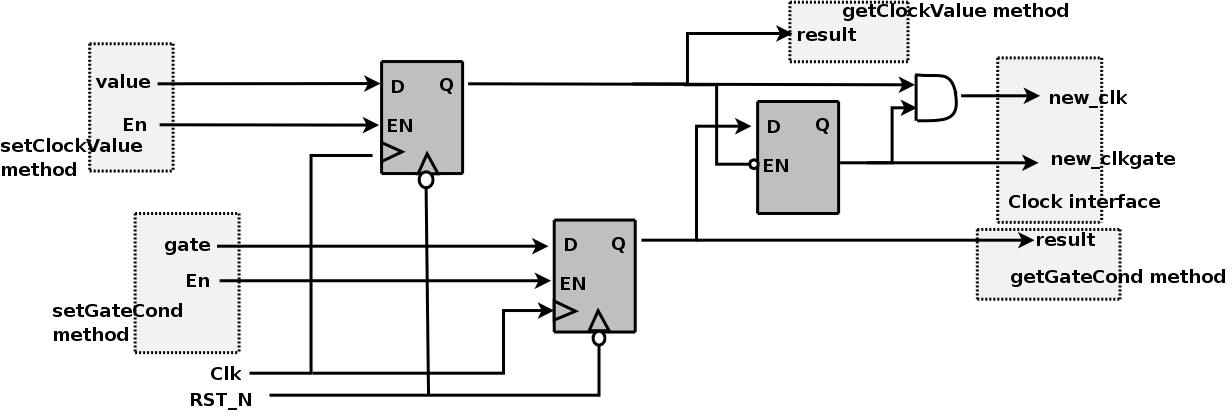
\includegraphics[width = 5 in]{LibFig/makeclock}
\caption{Clock Generator}
\label{makeclock}
\end{center}
\end{figure}


\index[function]{Clocks!mkClock}
\index{mkClock@\te{mkClock} (module)}
\begin{center}
\begin{tabular}{|p{1 in}|p{4.6 in}|}
\hline
&\\
\te{mkClock}&Creates a Clock type from a one-bit oscillator
input, and a Boolean gate condition.
There is no family relationship between the current clock and the clock
generated by this module.\\
\cline{2-2}
&\begin{libverbatim}
module mkClock #( one_bit_type initVal, Bool initGate) 
               ( MakeClockIfc#(one_bit_type) ifc )
   provisos( Bits#(one_bit_type, 1) ) ;
\end{libverbatim}
\\
\hline
\end{tabular}
\end{center}


\index[function]{Clocks!mkUngatedClock}
\index{mkUngatedClock@\te{mkUngatedClock} (module)}
\begin{center}
\begin{tabular}{|p{1 in}|p{4.6 in}|}
\hline
&\\
\te{mkUngatedClock}&Creates an ungated  Clock type from a one-bit oscillator
input.  There is no family relationship between the current clock and the clock
generated by this module.\\
\cline{2-2}
&\begin{libverbatim}
module mkUngatedClock #( one_bit_type initVal) 
               ( MakeClockIfc#(one_bit_type) ifc )
   provisos( Bits#(one_bit_type, 1) ) ;
\end{libverbatim}
\\
\hline
\end{tabular}
\end{center}

\index[function]{Clocks!mkGatedClock}
\index{mkGatedClock@\te{mkGatedClock} (module)}
 The \te{mkGatedClock} module adds (logic and) a Boolean gate condition
 to an existing clock, thus creating another clock in the same family.
 The source clock is provided as the argument \te{clk\_in}.
 The gate condition is controlled by an asynchronously-reset register
 inside the module.  The register is set with the \te{setGateCond} Action
 method of the interface and can be read with \te{getGateCond} method.
 The reset value of the gate condition register is provided as an
 instantiation parameter.  The clock for the register (and thus these set
 and get methods) is the default clock of the module; to specify a clock
 other than the default clock, use the \te{clocked\_by} directive.  

\begin{figure}[ht]
\begin{center}
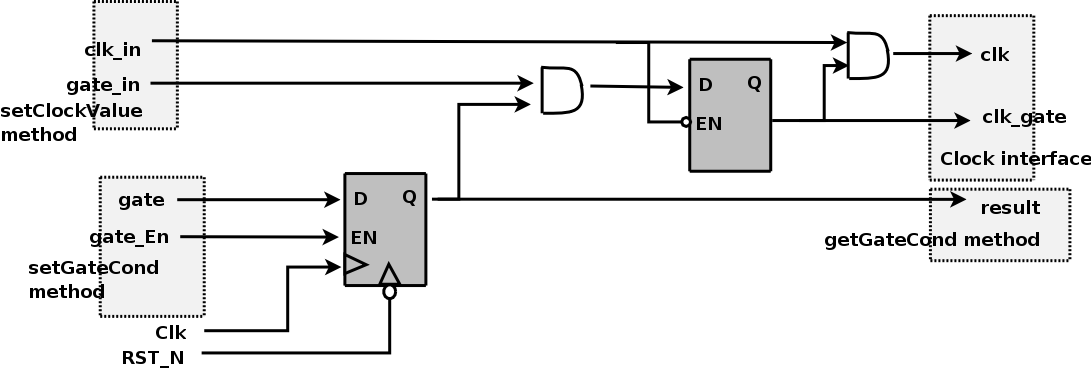
\includegraphics[width = 5 in]{LibFig/gatedclock}
\caption{Gated Clock Generator}
\label{gatedclock}
\end{center}
\end{figure}

\begin{center}
\begin{tabular}{|p{.9 in}|p{4.7 in}|}
\hline
& \\
\te{mkGatedClock}& Creates another clock in the same family by adding
logic and a Boolean gate condition to the current clock.\\
\cline{2-2}
&\begin{libverbatim}
module mkGatedClock#(Bool v) ( Clock clk_in, GatedClockIfc ifc );
\end{libverbatim}
\\ \hline
\end{tabular}
\end{center}

 For convenience, we provide an alternate version in which the source
 clock is the default clock of the module

\index[function]{Clocks!mkGatedClockFromCC}
\index{mkGatedClockFromCC@\te{mkGateClockFromCC} (module)}
\begin{center}
\begin{tabular}{|p{1.3 in}|p{4.3 in}|}
\hline
&\\
\te{mkGatedClockFromCC}&An alternate interface for the module
\te{mkGatedClock} in which the source clock is the default clock of
the module.\\
\cline{2-2}
&\begin{libverbatim}
module mkGatedClockFromCC#(Bool v) ( GatedClockIfc ifc );
\end{libverbatim}
\\
\hline
\end{tabular}
\end{center}

The modules \te{mkAbsoluteClock} and \te{mkAbsoluteClockFull}  provide
parametizable clock generation modules which are \emph{not}
synthesizable, but may be useful for testbenches.  In
\te{mkAbsoluteClock}, the first rising edge (start) and the
period are defined by parameters.  These parameters are measured in
Verilog delay times, which are usually specified during simulation
with the \te{timescale} directive.  Refer to the Verilog LRM for more
details on delay times. s Additional parameters are provided
by \te{mkAbsoluteClockFull}.  

\index{mkAbsoluteClock@\te{mkAbsoluteClock} (module)}
\index[function]{Clocks!mkAbsoluteClock}
\begin{center}
\begin{tabular}{|p{1.4 in}|p{4.2 in}|}
\hline
&\\
\te{mkAbsoluteClock}& The first rising edge (start) and period are
defined by parameters.  This module is not synthesizable.  \\
\cline{2-2}
&\begin{libverbatim}
module mkAbsoluteClock #( Integer start,
                          Integer period )
                          ( Clock );

\end{libverbatim}
\\
\hline
\end{tabular}
\end{center}

\index[function]{Clocks!mkAbsoluteClockFull}
\index{mkAbsoluteClockFull@\te{mkAbsoluteClockFull} (module)}
\begin{center}
\begin{tabular}{|p{1.4 in}|p{4.2 in}|}
\hline
&\\
\te{mkAbsoluteClockFull}& The value \te{initValue} is held until time \te{start}, and then the clock
oscillates.  The value \te{not(initValue)} is held for time
\te{compValTime}, followed by \te{initValue} held for time
\te{initValTime}.  Hence the clock period after startup is
\te{compValTime + initValTime}.   This module is not synthesizable.
 \\
\cline{2-2}
&\begin{libverbatim}
module mkAbsoluteClockFull #( Integer start, 
                              Bit#(1) initValue, 
                              Integer compValTime, 
                              Integer initValTime )
                              ( Clock );
\end{libverbatim}
\\
\hline
\end{tabular}
\end{center}



{\bf Verilog Modules}

The {\BSV} modules correspond to the following {\V}
modules, which are found in the BSC {\V} library, \te{\$BLUESPECDIR/Verilog/}.

\begin{center}
\begin{tabular}{|p {2.8 in}|p{2.8 in}|}
\hline
&\\
BSV Module Name & Verilog Module Name  \\
&\\
\hline
\hline
\te{mkAbsoluteClock}&\te{ClockGen.v} \\
\te{mkAbsoluteClockFull}& \\
\hline
\te{mkClock}&\te{MakeClock.v}\\
\te{mkUngatedClock}&\\
\hline
\te{mkGatedClock}&\te{GatedClock.v}\\
\te{mkGatedClockFromCC}&\\
\hline
\end{tabular}
\end{center}

%==========================================================================
\subsubsection{Clock Multiplexing}
\index{MuxClockIfc@\te{MuxClockIfc} (interface)}
\index{SelectClockIfc@\te{SelectClockIfc} (interface)}

{\bf Description}

BSC provides two gated clock multiplexing primitives:  a simple
combinational multiplexor and a stateful module which generates an
appropriate reset signal when the clock changes.  The first
multiplexor uses the interface \te{MuxClockIfc}, which  includes an
\te{Action} method to select the clock along with a \te{Clock}
subinterface.   The second multiplexor uses the interface
\te{SelectClockIfc} which also has  a \te{Reset} subinterface. 

Ungated versions of these modules are also provided.  The ungated
versions are identical to the gated versions, except that the input
and output clocks are ungated.  

{\bf Interfaces and Methods}

\begin{center}
\begin{tabular}{|p{.7in}|p{.7in}|p{1.8 in}|p{.4in}|p{1.4 in}|}
\hline
\multicolumn{5}{|c|}{MuxClockIfc Interface}\\
\hline
\multicolumn{3}{|c|}{Method and subinterfaces}&\multicolumn{2}{|c|}{Arguments}\\
\hline
Name & Type & Description& Name &\multicolumn{1}{|c|}{Description} \\
\hline
\hline 
\te{select}&\te{Action}&Method used to select the clock based on the
Boolean value {\tt ab} &{\tt ab}&if True, {\tt clock\_out} is taken
from {\tt aclk} \\
\hline
\te{clock\_out}&\te{Interface}&Clock interface&&\\
\hline
\end{tabular}
\end{center}


\begin{libverbatim}
     interface MuxClkIfc ;
        method    Action select ( Bool  ab ) ;
        interface Clock  clock_out ;
     endinterface
\end{libverbatim}

\begin{center}
\begin{tabular}{|p{.7in}|p{.7in}|p{1.8 in}|p{.4in}|p{1.4 in}|}
\hline
\multicolumn{5}{|c|}{SelectClockIfc Interface}\\
\hline
\multicolumn{3}{|c|}{Method and subinterfaces}&\multicolumn{2}{|c|}{Arguments}\\
\hline
Name & Type & Description& Name &\multicolumn{1}{|c|}{Description} \\
\hline
\hline 
\te{select}&\te{Action}&Method used to select the clock based on the
Boolean value {\tt ab} &{\tt ab}&if True, clock\_out is taken
from {\tt aclk} \\
\hline
\te{clock\_out}&\te{Interface}&Clock interface&&\\
\hline
\te{reset\_out}&\te{Interface}&Reset interface&&\\
\hline
\end{tabular}
\end{center}

\begin{libverbatim}
     interface SelectClkIfc ;
        method    Action select ( Bool  ab ) ;
        interface Clock  clock_out ;
        interface Reset  reset_out ;
     endinterface
\end{libverbatim}



{\bf Modules}

The \te{mkClockMux} module is a simple combinational multiplexor with
a registered clock selection signal,
which selects between clock inputs {\tt aClk} and {\tt bClk}.  The
provided  Verilog module
does not provide any glitch detection or removal logic;  it is the
responsibility of the user to provide additional logic to provide
glitch-free behavior.   The  \te{mkClockMux} module uses two
arguments and provides a Clock interface. The {\tt aClk} is selected if
{\tt ab} is True, while {\tt bClk} is selected otherwise.   

The \te{mkUngatedClockMux} module is identical to the \te{mkClockMux}
module except that the input and output clocks are ungated.  The
signals \te{aClkgate}, \te{bClkgate}, and \te{outClkgate} in figure
\ref{clockmux} don't exist.

\begin{figure}[ht]
\begin{center}
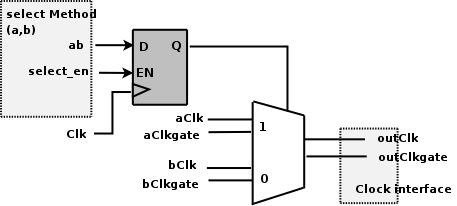
\includegraphics[height=1.4 in]{LibFig/clockmux}
\caption{Clock Multiplexor}
\label{clockmux}
\end{center}
\end{figure}


\index{mkClockMux@\te{mkClockMux} (module)}
\index[function]{Clocks!mkClockMux}
\begin{center}
\begin{tabular}{|p{1.4 in}|p{4.2 in}|}
\hline
&\\
\te{mkClockMux}&Simple combinational multiplexor,
which selects between aClk and bClk.\\
\cline{2-2}
&\begin{libverbatim}
module mkClockMux ( Clock aClk, Clock bClk )
                  ( MuxClkIfc ) ;
\end{libverbatim}
\\
\hline
\end{tabular}
\end{center}


\index{mkUngatedClockMux@\te{mkUngatedClockMux} (module)}
\index[function]{Clocks!mkUngatedClockMux}
\begin{center}
\begin{tabular}{|p{1.4 in}|p{4.2 in}|}
\hline
&\\
\te{mkUngatedClockMux}&Simple combinational multiplexor,
which selects between aClk and bClk.  None of the clocks are gated.\\
\cline{2-2}
&\begin{libverbatim}
module mkUngatedClockMux ( Clock aClk, Clock bClk )
                         ( MuxClkIfc ) ;
\end{libverbatim}
\\
\hline
\end{tabular}
\end{center}

\index{mkUngatedClockSelect@\te{mkUngatedClockSelect} (module)}
\index[function]{Clocks!mkUngatedClockSelect}
\index{mkClockSelect@\te{mkClockSelect} (module)}
\index[function]{Clocks!mkClockSelect}


The \te{mkClockSelect} module is a clock multiplexor 
containing additional logic which generates a reset whenever a new
clock is selected.  As such, the interface for the module includes
an \te{Action} method to select the clock (if {\tt ab} is True
clock\_out is taken from {\tt aClk}),
provides a \te{Clock} interface, and also a \te{Reset}
interface. 

The constructor for the module uses two clock arguments, and
provides the \te{MuxClockIfc} interface.  The underlying Verilog
module is {\tt ClockSelect.v};  it is expected that users can
substitute their own modules to meet any additional requirements
they may have.  The parameter {\tt stages} is the number of clock
cycles in which the reset is asserted after the clock selection changes.

The \te{mkUngatedClockSelect} module is identical to the \te{mkClockSelect}
module except that the input and output clocks are ungated.  The
signals \te{aClkgate}, \te{bClkgate}, and \te{outClk\_gate} in figure
\ref{clockselect} don't exist.


\begin{figure}[ht]
\begin{center}
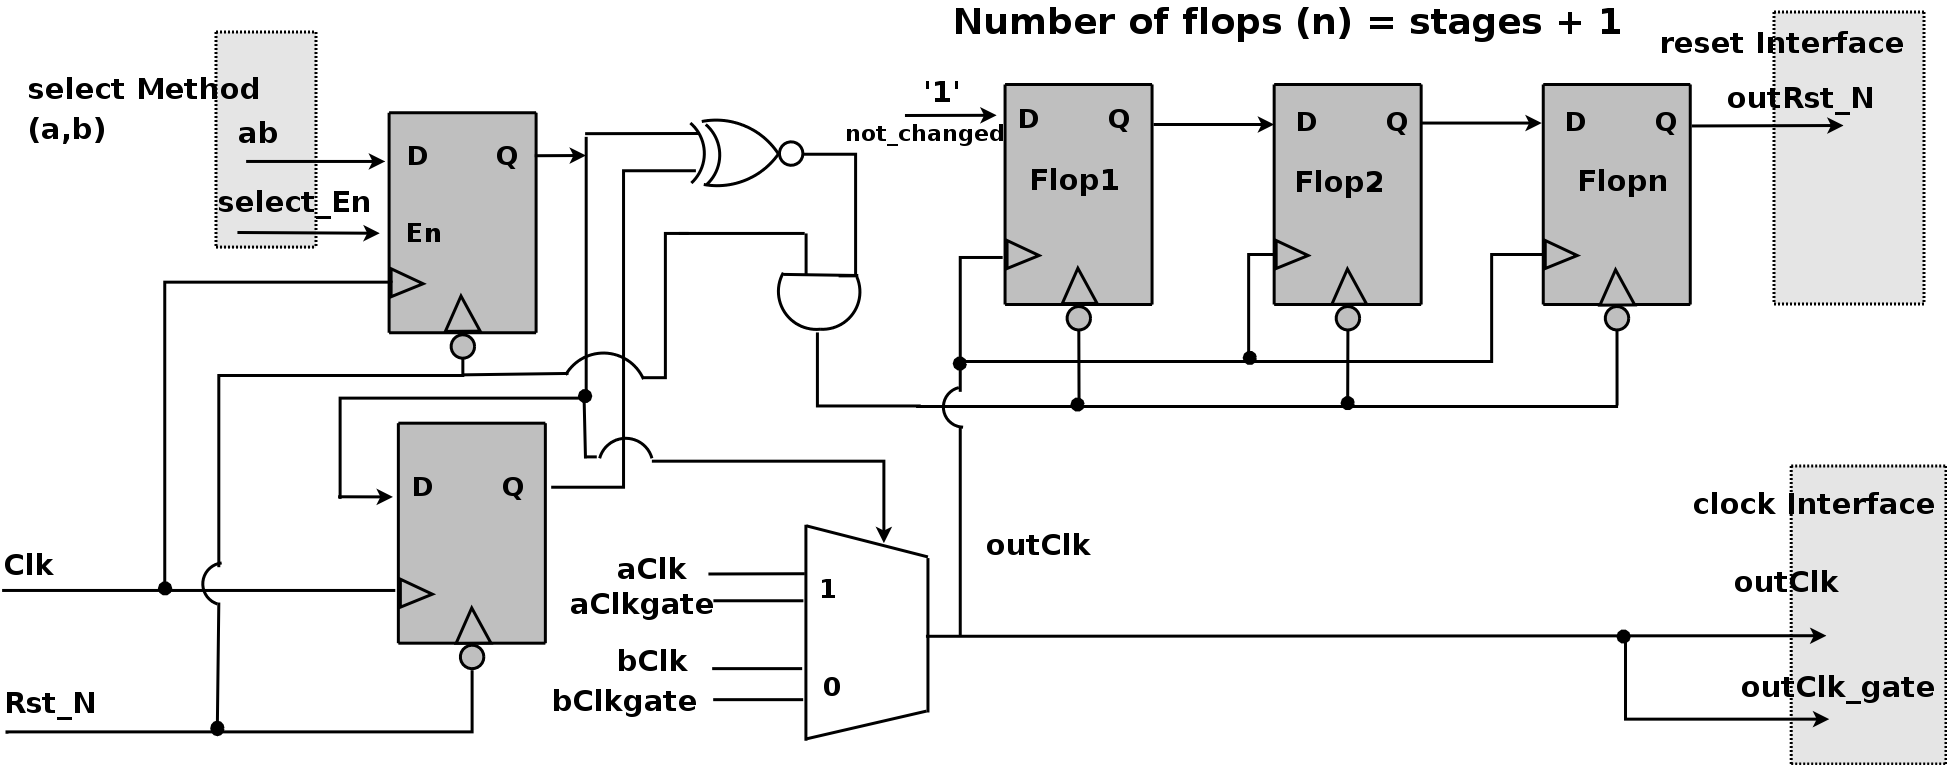
\includegraphics[width = 6 in]{LibFig/clockselect}
\caption{Clock Multiplexor with reset}
\label{clockselect}
\end{center}
\end{figure}



\begin{center}
\begin{tabular}{|p{1.4 in}|p{4.2 in}|}
\hline
&\\
\te{mkClockSelect}&Clock Multiplexor containing additional logic
which generates a reset whenever a new clock is selected.\\
\cline{2-2}
&\begin{libverbatim}
module mkClockSelect #( Integer stages, 
                          Clock aClk, 
                          Clock bClk, 
                        ( SelectClockIfc ) ;
\end{libverbatim}
\\
\hline
\end{tabular}
\end{center}      


\begin{center}
\begin{tabular}{|p{1.4 in}|p{4.2 in}|}
\hline
&\\
\te{mkUngatedClockSelect}&Clock Multiplexor containing additional logic
which generates a reset whenever a new clock is selected. The input
and output clocks are ungated.\\
\cline{2-2}
&\begin{libverbatim}
module mkUngatedClockSelect #( Integer stages, 
                               Clock aClk, 
                               Clock bClk, 
                             ( SelectClockIfc ) ;
\end{libverbatim}
\\
\hline
\end{tabular}
\end{center}      


   
{\bf Verilog Modules}

The {\BSV} modules correspond to the following {\V}
modules, which are found in the BSC {\V} library, \te{\$BLUESPECDIR/Verilog/}.


\begin{center}
\begin{tabular}{|p {2.8 in}|p{2.8 in}|}
\hline
&\\
BSV Module Name & Verilog Module Name  \\
&\\
\hline
\hline
\te{mkClockMux}& {\tt ClockMux.v} \\
\hline
\te{mkClockSelect}&{\tt ClockSelect.v}\\
\hline
\te{mkUngatedClockMux}& {\tt UngatedClockMux.v} \\
\hline
\te{mkUngatedClockSelect}&{\tt UngatedClockSelect.v}\\
\hline
\end{tabular}
\end{center}   
%======================================================================
\subsubsection{Clock Division}
\label{sec-clockdivider}
\index{ClockDividerIfc@\te{ClockDividerIfc} (interface)}
\index{mkClockDivider@\te{mkClockDivider} (module)}
\index{mkGatedClockDivider@\te{mkGatedClockDivider} (module)}
\index{mkClockDividerOffset@\te{mkClockDividerOffset} (module)}
\index{mkClockInverter@\te{mkClockInverter} (module)}
\index{mkGatedClockInverter@\te{mkGatedClockInverter} (module)}
\index[function]{Clocks!mkClockDivider}
\index[function]{Clocks!mkGatedClockDivider}
\index[function]{Clocks!mkClockInverter}
\index[function]{Clocks!mkGatedClockInverter}
\index[function]{Clocks!mkClockDividerOffset}
      
{\bf Description}

A clock divider provides a derived clock and also a \te{ClkNextRdy}
signal, which indicates that the divided
clock will rise in the next cycle.  This signal is associated with
the input clock, and can only be used within that clock domain.
     
The \te{AlignedFIFOs} package (Section \ref{sec-AlignedFIFOs})
contains parameterized FIFO modules for 
creating synchronizing FIFOs between clock domains with aligned edges.

% See {\tt mkSyncRegToSlow}, {\tt mkSyncRegToFast}, {\tt
%  mkSyncFIFOToSlow}, and {\tt mkSyncFIFOToFast} in Section
%  \ref{crossing-prim}
%  for some specialized synchronizers
% which can be used with divided clocks, and other systems when the
% clock edges are known to be aligned.
      
{\bf Data Types}

The \te{ClkNextRdy} is a Boolean 
signal which indicates that the slow
clock will rise in the next cycle.

\begin{libverbatim}
     typedef Bool ClkNextRdy ;
\end{libverbatim}

{\bf Interfaces and Methods}

\begin{center}
\begin{tabular}{|p{.7in}|p{.7in}|p{3.6 in}|}
\hline
\multicolumn{3}{|c|}{ClockDividerIfc Interface}\\
\hline
Name & Type & Description\\
\hline
\hline 
\te{fastClock}&\te{Interface}&The original clock\\
\hline
\te{slowClock}&\te{Interface}&The derived clock\\
\hline
\te{clockReady}&\te{Bool}&Boolean value which indicates that the
slow clock will rise in the next cycle.  The method is in the clock
domain of the fast clock.\\
\hline
\end{tabular}
\end{center}

\begin{libverbatim}
     interface ClockDividerIfc ;
         interface Clock      fastClock ;           
         interface Clock      slowClock ;           
         method    ClkNextRdy clockReady() ;        
     endinterface 
\end{libverbatim}

{\bf Modules}

The {\tt divider} parameter may be any integer greater than 1.
For even dividers the generated clock's duty cycle is 50\%, while
for odd dividers, the duty cycle is $(divider/2) / divider$.  Since
\te{divisor} is an integer, the remainder is truncated when divided.   The
current clock (or the \te{clocked\_by} argument) is used as the
source clock.  

\begin{figure}[ht]
\begin{center}
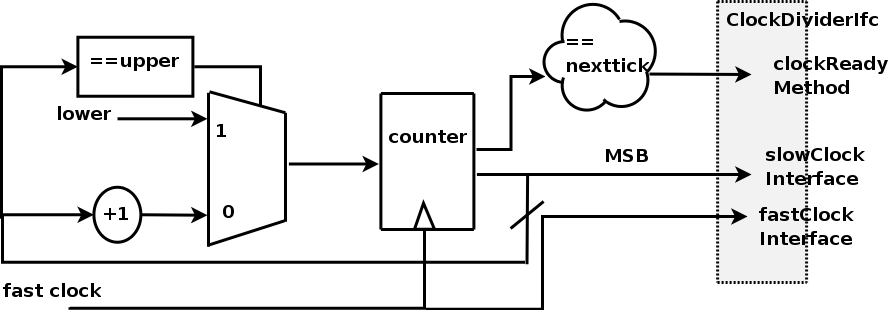
\includegraphics[height=1.2 in]{LibFig/clockdiv}
\caption{Clock Divider}
\label{clockdiv}
\end{center}
\end{figure}


\begin{center}
\begin{tabular}{|p{1.6 in}|p{4.0 in}|}
\hline
&\\
\te{mkClockDivider}& Basic clock divider.\\
\cline{2-2}
&\begin{libverbatim}
module mkClockDivider #( Integer divisor ) 
                       ( ClockDividerIfc ) ;
\end{libverbatim}
\\
\hline
\end{tabular}
\end{center}


\begin{center}
\begin{tabular}{|p{1.6 in}|p{4.0 in}|}
\hline
&\\
\te{mkGatedClockDivider}& A gated verison of the basic clock divider.\\
\cline{2-2}
&\begin{libverbatim}
module mkGatedClockDivider #( Integer divisor 
                            )( ClockDividerIfc ) ;
\end{libverbatim}
\\
\hline
\end{tabular}
\end{center}



The {\tt  mkClockDividerOffset} module provides a clock divider 
where the rising edge can be defined relative to other clock
dividers which have the same divisor.  An offset of value 2 will
produce a rising edge one fast clock after a divider with offset
1.  \te{mkClockDivider} is just \te{mkClockDividerOffset} with an
offset of value 0. 

\begin{center}
\begin{tabular}{|p{1.6 in}|p{4.0 in}|}
\hline
&\\
\te{mkClockDividerOffset}&Provides a clock divider,
where the rising edge can be defined relative to other clock
dividers which have the same divisor.\\
\cline{2-2}
&\begin{libverbatim}
module mkClockDividerOffset #( Integer divisor, 
                               Integer offset )
                             ( ClockDividerIfc ) ;
\end{libverbatim}
\\
\hline
\end{tabular}
\end{center}


The \te{mkClockInverter} and \te{mkGatedClockInverter} modules
generate an inverted clock having the same period but opposite phase
as the current clock.  The \te{mkGatedClockInverter} is a gated
version of \te{mkClockInverter}.  The output
clock includes a gate signal derived from the gate of the input clock.
 
\begin{center}
\begin{tabular}{|p{1.6 in}|p{4.0 in}|}
\hline
&\\
\te{mkClockInverter}&Generates an inverted clock having
the same period but opposite phase as the current clock.\\
\cline{2-2}
&\begin{libverbatim}
module mkClockInverter ( ClockDividerIfc ) ;
\end{libverbatim}     
\\
\hline
\end{tabular}
\end{center} 


\begin{center}
\begin{tabular}{|p{1.6 in}|p{4.0 in}|}
\hline
&\\
\te{mkGatedClockInverter}&A gated version of \te{mkClockInverter}.
\\
\cline{2-2}
&\begin{libverbatim}
module mkGatedClockInverter ( ClockDividerIfc ifc ) ;
\end{libverbatim}     
\\
\hline
\end{tabular}
\end{center} 

{\bf Verilog Modules}

The {\BSV} modules correspond to the following {\V}
modules, which are found in the BSC {\V} library, \te{\$BLUESPECDIR/Verilog/}.


\begin{center}
\begin{tabular}{|p {2.8 in}|p{2.8 in}|}
\hline
&\\
BSV Module Name & Verilog Module Name  \\
&\\
\hline
\hline
{\tt mkClockDivider}& \te{ClockDiv.v}\\
{\tt mkClockDividerOffset}&\\
\hline
{\tt mkGatedClockDivider}&\te{GatedClockDiv.v}\\
\hline
{\tt mkClockInverter}&\te{ClockInverter.v}\\
\hline
{\tt mkGatedClockInverter}&\te{GatedClockInverter.v}\\
\hline
\end{tabular}
\end{center}

%=====================================================================
\subsubsection{Bit Synchronizers}

\index{SyncBitIfc@\te{SyncBitIfc} (interface)}

{\bf Description}

Bit synchronizers are used to safely transfer one bit of data from one
clock domain to another.  More complicated synchronizers are provided
in later sections.

{\bf Interfaces and Methods}

The  {\tt SyncBitIfc} interface provides a \te{send} method
which  transmits
one bit of information from one clock domain to the \te{read}
method in a second domain.

\begin{center}
\begin{tabular}{|p{.4in}|p{.8 in}|p{1.8 in}|p{.6in}|p{1.4 in}|}
\hline
\multicolumn{5}{|c|}{SyncBitIfc Interface}\\
\hline
\multicolumn{3}{|c|}{Methods}&\multicolumn{2}{|c|}{Arguments}\\
\hline
Name & Type & Description& Name &\multicolumn{1}{|c|}{Description} \\
\hline
\hline 
\te{send}&\te{Action}&Transmits information from one clock
domain to the second domain&\te{bitData}&One bit of information transmitted \\
\hline
\te{read}&\te{one\_bit\_type}&Reads one bit of data sent from a
different clock domain&&\\
\hline
\end{tabular}
\end{center}


\begin{libverbatim}
     interface SyncBitIfc #(type one_bit_type) ;
        method Action       send ( one_bit_type bitData ) ;
        method one_bit_type read () ;
     endinterface
\end{libverbatim}



{\bf Modules}

The \te{mkSyncBit}, \te{mkSyncBitFromCC} and \te{mkSyncBitToCC}
modules provide a \te{SyncBitIfc} across clock domains.  The send
method is in  one clock domain, and the read method is in
a second clock domain, as shown in Figure \ref{bitsynch}.  The
\te{FromCC}  and \te{ToCC} versions
differ in that the \te{FromCC} module moves data {\em{from}} the current clock
(module's clock), while
the \te{ToCC} module moves data {\em{to}} the current clock domain.
The  hardware implementation is a two
register synchronizer, which can be found in \te{SyncBit.v} in the
BSC {\V} library directory.
 

\begin{figure}[ht]
\begin{center}
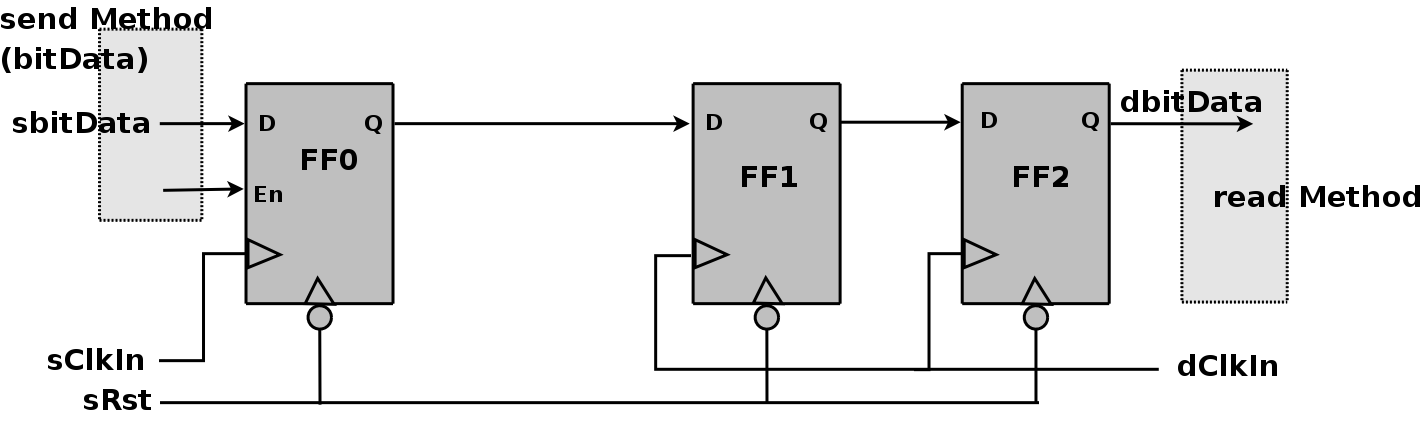
\includegraphics[height=1.2 in]{LibFig/bitsynch}
\caption{Bit Synchronizer}
\label{bitsynch}
\end{center}
\end{figure}


\index{mkSyncBit@\te{mkSyncBit} (module)}
\index[function]{Clocks!mkSyncBit}
\begin{center}
\begin{tabular}{|p{1.4 in}|p{4.2 in}|}
\hline
&\\
\te{mkSyncBit}&Moves data across clock domains.  The in and out clocks,
along with the input reset, are explicitly provided.  The default clock
and reset are ignored.\\
\cline{2-2}
&\begin{libverbatim}
module mkSyncBit #( Clock sClkIn, Reset sRst, 
                    Clock dClkIn ) 
                  ( SyncBitIfc #(one_bit_type) )
   provisos( Bits#(one_bit_type, 1)) ;
\end{libverbatim}     
\\
\hline
\end{tabular}
\end{center} 

\index[function]{Clocks!mkSyncBitFromCC}
\index{mkSyncBitFromCC@\te{mkSyncBitFromCC} (module)}
\begin{center}
\begin{tabular}{|p{1.4 in}|p{4.2 in}|}
\hline
&\\
\te{mkSyncBitFromCC}&Moves data from the current clock (the module's
clock) to a different clock domain. The input clock and reset are the
current clock and reset.  \\
\cline{2-2}
&\begin{libverbatim}
module mkSyncBitFromCC #( Clock dClkIn )
                        ( SyncBitIfc #(one_bit_type) ) 
   provisos( Bits#(one_bit_type, 1)) ;
\end{libverbatim}     
\\
\hline
\end{tabular}
\end{center} 

\index[function]{Clocks!mkSyncBitToCC}
\index{mkSyncBitToCC@\te{mkSyncBitToCC} (module)}
\begin{center}
\begin{tabular}{|p{1.4 in}|p{4.2 in}|}
\hline
&\\
\te{mkSyncBitToCC}&Moves data into the current clock domain. The
output clock is the current clock. The current reset is ignored. \\
\cline{2-2}
&\begin{libverbatim}
module mkSyncBitToCC #( Clock sClkIn, Reset sRstIn )
                      ( SyncBitIfc #(one_bit_type) ) 
   provisos( Bits#(one_bit_type, 1)) ;
\end{libverbatim}     
\\
\hline
\end{tabular}
\end{center} 

\index[function]{Clocks!mkSyncBit15}
\index{mkSyncBit15@\te{mkSyncBit15} (module)}
The \te{mkSyncBit15} module (one and a half) and its variants provide the same
interface as the \te{mkSyncBit} modules, but the underlying
hardware is slightly modified, as shown in Figure \ref{bitsynch15}. For these synchronizers, the first
register clocked by the destination clock triggers on the falling
edge of the clock.  
   
\begin{figure}[ht]
\begin{center}
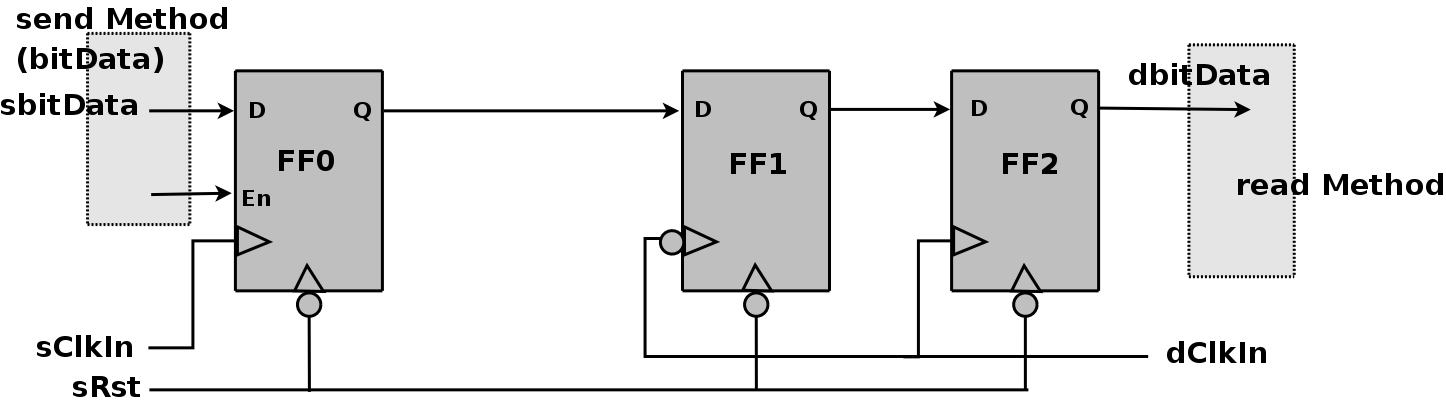
\includegraphics[height=1.2 in]{LibFig/bitsynch15}
\caption{Bit Synchronizer 1.5 - first register in destination domain
triggers  on falling edge}
\label{bitsynch15}
\end{center}
\end{figure}


\begin{center}
\begin{tabular}{|p{1.4 in}|p{4.2 in}|}
\hline
&\\
\te{mkSyncBit15}&Similar to \te{mkSyncBit} except it
 triggers on the falling edge of the clock. The in and out clocks,
along with the input reset, are explicitly provided.  The default clock
and reset are ignored.   \\
\cline{2-2}
&\begin{libverbatim}
module mkSyncBit15 #( Clock sClkIn, Reset sRst, 
                      Clock dClkIn )
                    ( SyncBitIfc #(one_bit_type) ) 
   provisos( Bits#(one_bit_type, 1)) ;
\end{libverbatim}     
\\
\hline
\end{tabular}
\end{center} 

\index[function]{Clocks!mkSyncBit15FromCC}
\index{mkSyncBit15FromCC@\te{mkSyncBit15FromCC} (module)}
\begin{center}
\begin{tabular}{|p{1.4 in}|p{4.2 in}|}
\hline
&\\
\te{mkSyncBit15FromCC}&Moves data from the current clock and is
triggered on the falling edge of the clock. The input clock and reset are the
current clock and reset. \\
\cline{2-2}
&\begin{libverbatim}
module mkSyncBit15FromCC #(Clock dClkIn)
                          (SyncBitIfc #(one_bit_type)) 
   provisos( Bits#(one_bit_type, 1)) ;
\end{libverbatim}     
\\
\hline
\end{tabular}
\end{center} 

\index[function]{Clocks!mkSyncBit15ToCC}
\index{mkSyncBit15ToCC@\te{mkSyncBit15ToCC} (module)}
\begin{center}
\begin{tabular}{|p{1.4 in}|p{4.2 in}|}
\hline
&\\
\te{mkSyncBit15ToCC}&Moves data into the current clock domain and is
triggered on the falling edge of the clock. The
output clock is the current clock. The current reset is ignored. \\
\cline{2-2}
&\begin{libverbatim}
module mkSyncBit15ToCC #( Clock sClkIn, Reset sRstIn )
                        ( SyncBitIfc #(one_bit_type) ) 
   provisos( Bits#(one_bit_type, 1)) ;
\end{libverbatim}     
\\
\hline
\end{tabular}
\end{center} 

\index[function]{Clocks!mkSyncBit1}
\index{mkSyncBit1@\te{mkSyncBit1} (module)}
The \te{mkSyncBit1} module, shown in Figure \ref{bitsynch1}, also
provides the  same interface but
only uses one register in the destination domain.  Synchronizers
like this, which use only one
register, are not generally used since meta-stable output
is more probable.  However, one can use this synchronizer provided
special meta-stable resistant flops are selected during physical
synthesis or (for example) if the output is immediately registered.

\begin{figure}[ht]
\begin{center}
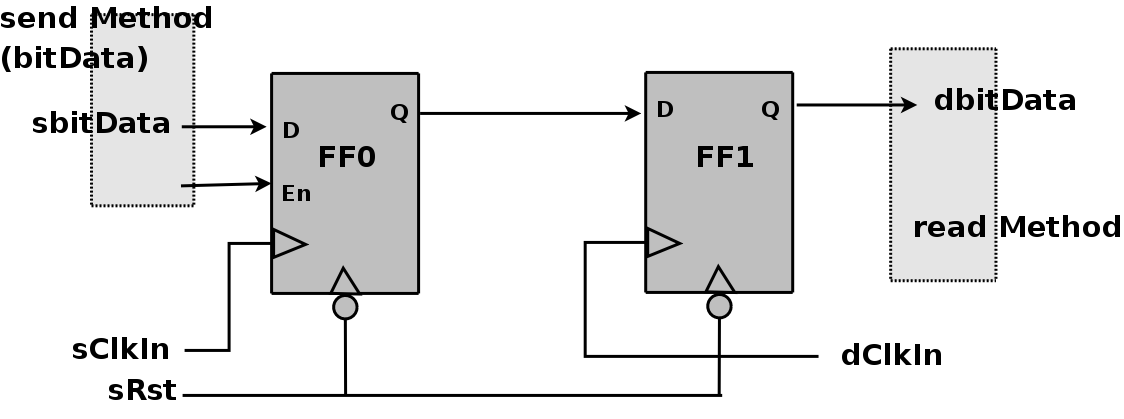
\includegraphics[height=1.2 in]{LibFig/bitsynch1}
\caption{Bit Synchronizer 1.0 - single register in destination domain}
\label{bitsynch1}
\end{center}
\end{figure}



\begin{center}
\begin{tabular}{|p{1.4 in}|p{4.2 in}|}
\hline
&\\
\te{mkSyncBit1}&Moves data from one clock domain to another clock
domain, with only one register in the destination domain. The in and out clocks,
along with the input reset, are explicitly provided.  The default clock
and reset are ignored. \\
\cline{2-2}
&\begin{libverbatim}
module mkSyncBit1 #( Clock sClkIn, Reset sRst,
                     Clock dClkIn )
                   ( SyncBitIfc #(one_bit_type) ) 
   provisos( Bits#(one_bit_type, 1)) ;
\end{libverbatim}     
\\
\hline
\end{tabular}
\end{center} 


\index[function]{Clocks!mkSyncBit1FromCC}
\index{mkSyncBit1FromCC@\te{mkSyncBit1FromCC} (module)}
\begin{center}
\begin{tabular}{|p{1.4 in}|p{4.2 in}|}
\hline
&\\
\te{mkSyncBit1FromCC}&Moves data from the current clock domain, with only one register in the destination domain. The input clock and reset are the
current clock and reset. \\
\cline{2-2}
&\begin{libverbatim}
module mkSyncBit1FromCC #( Clock dClkIn )
                         ( SyncBitIfc #(one_bit_type) ) 
   provisos( Bits #(one_bit_type, 1)) ;
\end{libverbatim}     
\\
\hline
\end{tabular}
\end{center} 

\index[function]{Clocks!mkSyncBit1ToCC}
\index{mkSyncBit1ToCC@\te{mkSyncBit1ToCC} (module)}
\begin{center}
\begin{tabular}{|p{1.4 in}|p{4.2 in}|}
\hline
&\\
\te{mkSyncBit1ToCC}& Moves data into the current clock domain, with
only one register in the destination domain. The
output clock is the current clock. The current reset is ignored.  \\
\cline{2-2}
&\begin{libverbatim}
module mkSyncBit1ToCC #( Clock sClkIn, Reset sRstIn )
                       ( SyncBitIfc #(one_bit_type) ) 
   provisos( Bits#(one_bit_type, 1)) ;
\end{libverbatim}     
\\
\hline
\end{tabular}
\end{center} 

%// A general module which not use the current clock or reset


The \te{mkSyncBit05} module is similar to \te{mkSyncBit1}, but the
destination  register
triggers on the falling edge of the clock, as shown in Figure \ref{bitsynch05}.


\begin{figure}[ht]
\begin{center}
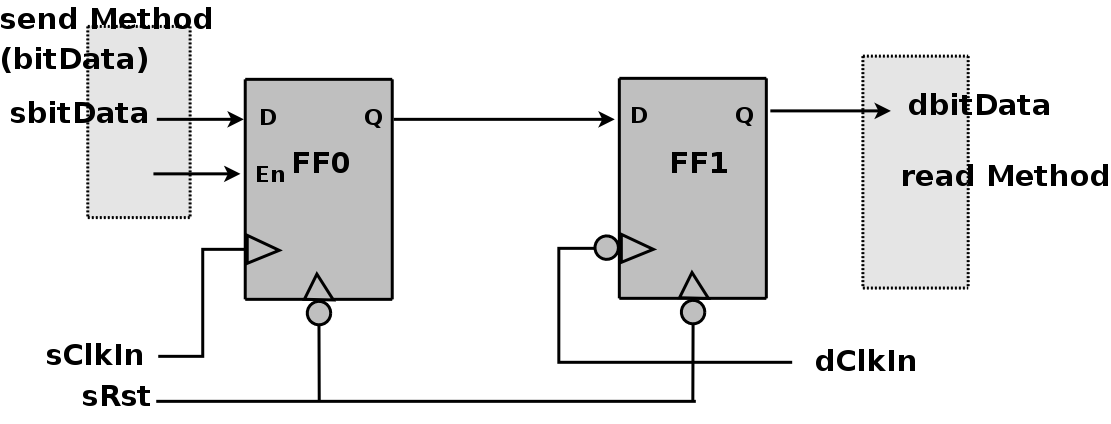
\includegraphics[height=1.2 in]{LibFig/bitsynch05}
\caption{Bit Synchronizer .5 - first register in destination domain
triggers on falling edge}
\label{bitsynch05}
\end{center}
\end{figure}

\index[function]{Clocks!mkSyncBit05}
\index{mkSyncBit05@\te{mkSyncBit05} (module)}
\begin{center}
\begin{tabular}{|p{1.4 in}|p{4.2 in}|}
\hline
&\\
\te{mkSyncBit05}&Moves data from one clock domain to another clock
domain, with only one register in the destination domain.  The destination register triggers on the falling edge of the clock. The in and out clocks,
along with the input reset, are explicitly provided.  The default clock
and reset are ignored.\\
\cline{2-2}
&\begin{libverbatim}
module mkSyncBit05 #( Clock sClkIn, Reset sRst, 
                      Clock dClkIn ) 
                    ( SyncBitIfc #(one_bit_type) ) 
   provisos( Bits#(one_bit_type, 1)) ;
\end{libverbatim}     
\\
\hline
\end{tabular}
\end{center} 

\index[function]{Clocks!mkSyncBit05FromCC}
\index{mkSyncBit05FromCC@\te{mkSyncBit05FromCC} (module)}   
\begin{center}
\begin{tabular}{|p{1.4 in}|p{4.2 in}|}
\hline
&\\
\te{mkSyncBit05FromCC}&Moves data from the current clock domain, with only one register
in the destination domain, the destination register triggers on the
falling edge of the clock.   The input clock and reset are the
current clock and reset.  \\
\cline{2-2}
&\begin{libverbatim}
module mkSyncBit05FromCC #( Clock dClkIn ) 
                          (SyncBitIfc #(one_bit_type) ) 
   provisos( Bits#(one_bit_type, 1)) ;
\end{libverbatim}     
\\
\hline
\end{tabular}
\end{center} 

\index[function]{Clocks!mkSyncBit05ToCC}
\index{mkSyncBit05ToCC@\te{mkSyncBit05ToCC} (module)}
\begin{center}
\begin{tabular}{|p{1.4 in}|p{4.2 in}|}
\hline
&\\
\te{mkSyncBit05ToCC}&Moves data into the current clock domain, with only one register
in the destination domain, the destination register triggers on the
falling edge of the clock.  The
output clock is the current clock. The current reset is ignored.    \\
\cline{2-2}
&\begin{libverbatim}
module mkSyncBit05ToCC #( Clock sClkIn, Reset sRstIn ) 
                        ( SyncBitIfc #(one_bit_type) ) 
   provisos( Bits#(one_bit_type, 1)) ;
\end{libverbatim}     
\\
\hline
\end{tabular}
\end{center} 

{\bf Verilog Modules}

The {\BSV} modules correspond to the following {\V}
modules, which are found in the BSC {\V} library, \te{\$BLUESPECDIR/Verilog/}.


\begin{center}
\begin{tabular}{|p {2.8 in}|p{2.8 in}|}
\hline
&\\
BSV Module Name & Verilog Module Name  \\
&\\
\hline
\hline
\te{mkSyncBit}& \te{SyncBit.v}\\
\te{mkSyncBitFromCC}&\\
\te{mkSyncBitToCC}&\\
\hline
\te{mkSyncBit15}&\te{SyncBit15.v}\\
\te{mkSyncBit15FromCC}&\\
\te{mkSyncBit15ToCC}&\\
\hline
\te{mkSyncBit1}&\te{SyncBit1.v}\\
\te{mkSyncBit1FromCC}&\\
\te{mkSyncBit1ToCC}&\\
\hline
\te{mkSyncBit05}&\te{SyncBit05.v}\\
\te{mkSyncBit05FromCC}&\\
\te{mkSyncBit05ToCC}&\\
\hline
\end{tabular}
\end{center}
%====================================================
\subsubsection{Pulse Synchronizers}
\index{SyncPulseIfc@\te{SyncPulseIfc} (interface)}

{\bf Description}

Pulse synchronizers are used to transfer a pulse from one clock domain
to another.


{\bf Interfaces and Methods}

The \te{SyncPulseIfc} interface provides an Action method, \te{send},
which  when
invoked generates a True value on the \te{pulse} method in a second clock domain.

\begin{center}
\begin{tabular}{|p{.4in}|p{.8 in}|p{3.6in}|}
\hline
\multicolumn{3}{|c|}{SyncPulseIfc Interface}\\
\hline
\multicolumn{3}{|c|}{Methods}\\
\hline
Name & Type & Description\\
\hline
\hline 
\te{send}&\te{Action}&Starts transmittling a pulse from one clock
domain to the second clock domain.\\
\hline
\te{pulse}&\te{Bool}&Where the pulse is received in the second domain.
\te{pulse} is True if a pulse is recieved in this cycle.\\
\hline
\end{tabular}
\end{center}

\begin{libverbatim}
     interface SyncPulseIfc ;
        method Action send  () ;
        method Bool   pulse () ;
     endinterface
\end{libverbatim}

{\bf Modules}

The \te{mkSyncPulse}, \te{mkSyncPulseFromCC} and \te{mkSyncPulseToCC} modules
provide clock domain crossing modules for pulses.  When the
\te{send} method is called from the one clock domain, a pulse will
be seen on the \te{read} method in the second.  Note that there is
no handshaking between the domains, so when sending data
from a fast clock domain to a slower one, not all pulses sent may
be seen in the slower receiving clock domain.  The pulse delay is
two destination clocks cycles.

\begin{figure}[ht]
\begin{center}
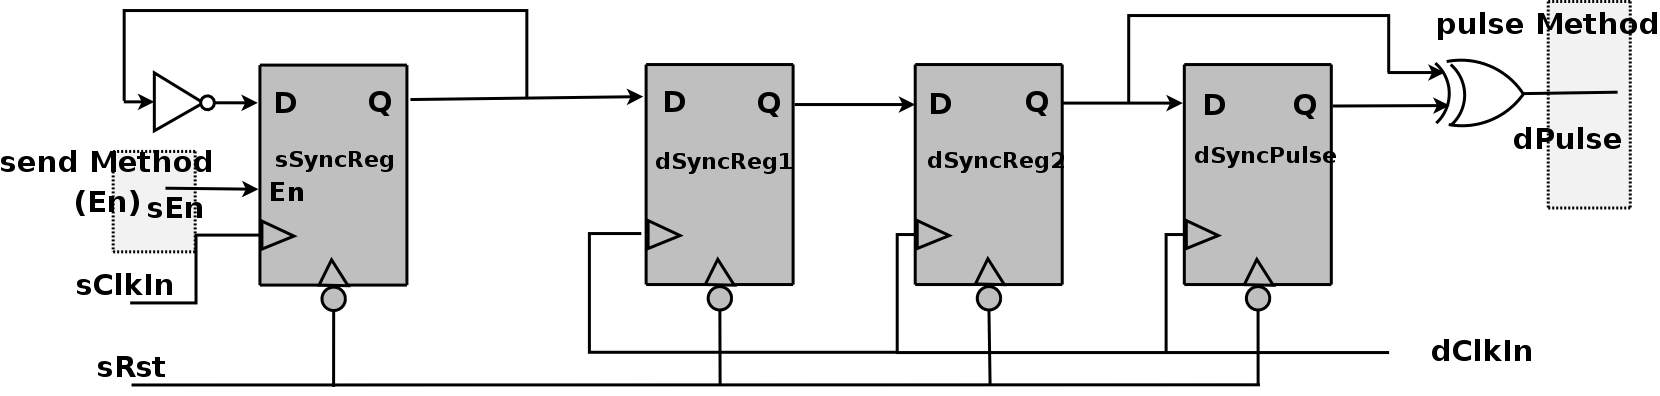
\includegraphics[width = 5 in]{LibFig/syncpulse}
\caption{Pulse Synchronizer - no handshake}
\label{syncpulse}
\end{center}
\end{figure}

\index[function]{Clocks!mkSyncPulse}
\index{mkSyncPulse@\te{mkSyncPulse} (module)}
\begin{center}
\begin{tabular}{|p{1.4 in}|p{4.2 in}|}
\hline
&\\
\te{mkSyncPulse}&Sends a pulse from one clock domain to another. The in and out clocks,
along with the input reset, are explicitly provided.  The default clock
and reset are ignored. \\
\cline{2-2}
&\begin{libverbatim}
module mkSyncPulse #( Clock sClkIn, Reset sRstIn, 
                      Clock dClkIn )
                    ( SyncPulseIfc ) ;
\end{libverbatim}     
\\
\hline
\end{tabular}
\end{center} 

\index[function]{Clocks!mkSyncPulseFromCC}
\index{mkSyncPulseFromCC@\te{mkSyncPulseFromCC} (module)}
\begin{center}
\begin{tabular}{|p{1.4 in}|p{4.2 in}|}
\hline
&\\
\te{mkSyncPulseFromCC}&Sends a pulse from the current clock domain to
the other clock domain. The input clock and reset are the
current clock and reset. \\
\cline{2-2}
&\begin{libverbatim}
module mkSyncPulseFromCC #( Clock dClkIn ) 
                          ( SyncPulseIfc ) ;
\end{libverbatim}     
\\
\hline
\end{tabular}
\end{center} 

\index[function]{Clocks!mkSyncPulseToCC}
\index{mkSyncPulseToCC@\te{mkSyncPulseToCC} (module)}
\begin{center}
\begin{tabular}{|p{1.4 in}|p{4.2 in}|}
\hline
&\\
\te{mkSyncPulseToCC}&Sends a pulse from the other clock domain to the
current clock domain.  The
output clock is the current clock. The current reset is ignored.  \\
\cline{2-2}
&\begin{libverbatim}
module mkSyncPulseToCC #( Clock sClkIn, Reset sRstIn ) 
                        ( SyncPulseIfc ) ;
\end{libverbatim}     
\\
\hline
\end{tabular}
\end{center} 

%\index[function]{Clocks!mkSyncHandshake}
%\index{mkSyncHandshake@\te{mkSyncHandshake} (module)}
The \te{mkSyncHandshake}, \te{mkSyncHandshakeFromCC} and \te{mkSyncHandshakeToCC} modules
provide clock domain crossing modules for pulses in a similar way
as \te{mkSyncPulse} modules, except that a handshake is provided
in the \te{mkSyncHandshake} versions. The handshake enforces that
another send does not occur before the first pulse crosses to the
other domain.  Note that this only guarantees that the pulse is seen
in one clock cycle of the destination; it does not guarantee that the
system on that side reacted to the pulse before it was gone.  It is up
to the designer to ensure this, if necessary.  The modules are not
ready in reset. 

The pulse delay from the \te{send} method to the \te{read} method
is two destination clocks.  The \te{send} method is re-enabled in
two destination clock cycles plus two source clock cycles after the
\te{send} method is called.  




\begin{figure}[ht]
\begin{center}
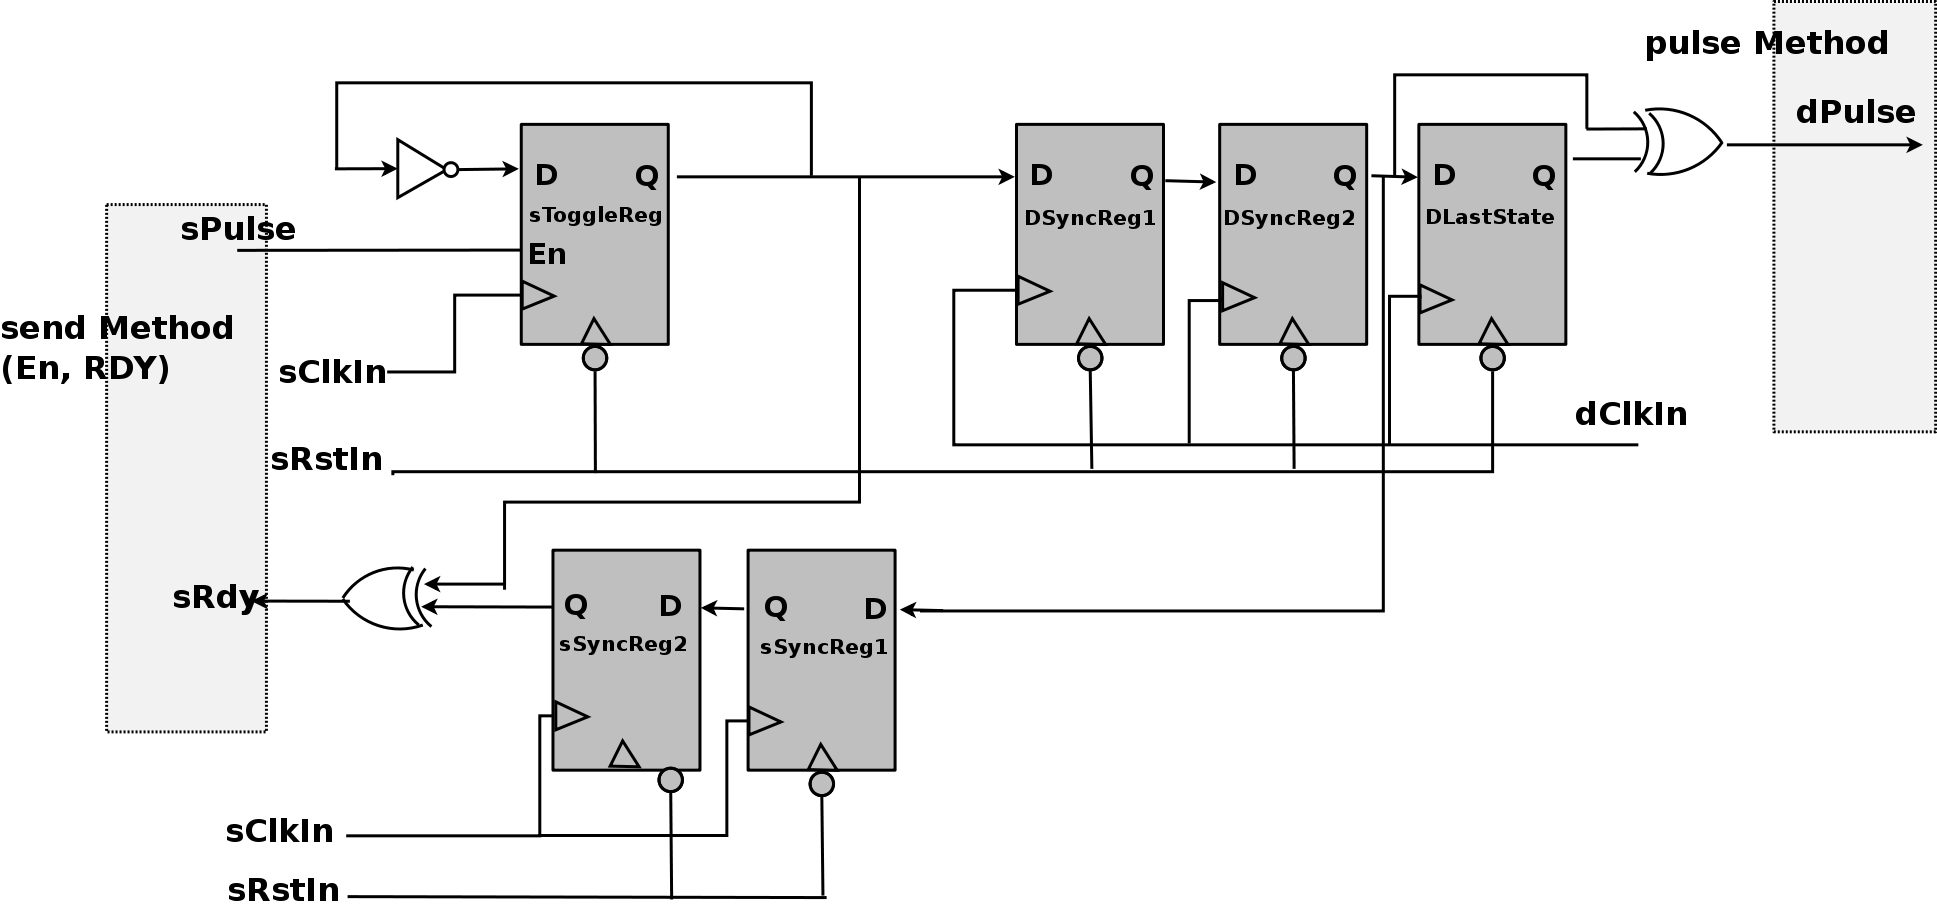
\includegraphics[width = 5.5 in]{LibFig/synchandshake}
\caption{Pulse Synchronizer with handshake}
\label{synchandshake}
\end{center}
\end{figure}


\index[function]{Clocks!mkSyncHandshake}
\index{mkSyncHandshake@\te{mkSyncHandshake} (module)}
\begin{center}
\begin{tabular}{|p{1.4 in}|p{4.2 in}|}
\hline
&\\
\te{mkSyncHandshake}&Sends a pulse from one clock domain to another
clock domain with handshaking.  The in and out clocks,
along with the input reset, are explicitly provided.  The default clock
and reset are ignored.  \\
\cline{2-2}
&\begin{libverbatim}
module mkSyncHandshake #( Clock sClkIn, Reset sRstIn, 
                          Clock dClkIn )
                        ( SyncPulseIfc ) ;
\end{libverbatim}     
\\
\hline
\end{tabular}
\end{center} 

\index[function]{Clocks!mkSyncHandshakeFromCC}
\index{mkSyncHandshakeFromCC@\te{mkSyncHandshakeFromCC} (module)}
\begin{center}
\begin{tabular}{|p{1.6 in}|p{4.0 in}|}
\hline
&\\
\te{mkSyncHandshakeFromCC}&Sends a pulse with a handshake from the
current clock domain. The input clock and reset are the
current clock and reset. \\
\cline{2-2}
&\begin{libverbatim}
module mkSyncHandshakeFromCC #( Clock dClkIn ) 
                              ( SyncPulseIfc ) ;
\end{libverbatim}     
\\
\hline
\end{tabular}
\end{center} 

\index[function]{Clocks!mkSyncHandshakeToCC}
\index{mkSyncHandshakeToCC@\te{mkSyncHandshakeToCC} (module)}
\begin{center}
\begin{tabular}{|p{1.6 in}|p{4.0 in}|}
\hline
&\\
\te{mkSyncHandshakeToCC}&Sends a pulse with a handshake to the current
clock domain.  The
output clock is the current clock. The current reset is ignored. \\
\cline{2-2}
&\begin{libverbatim}
module mkSyncHandshakeToCC #( Clock sClkIn, 
                              Reset sRstIn )
                            ( SyncPulseIfc ) ;
\end{libverbatim}     
\\
\hline
\end{tabular}
\end{center} 

{\bf Verilog Modules}

The {\BSV} modules correspond to the following {\V}
modules, which are found in the BSC {\V} library, \te{\$BLUESPECDIR/Verilog/}.

\begin{center}
\begin{tabular}{|p {2.8 in}|p{2.8 in}|}
\hline
&\\
BSV Module Name & Verilog Module Name  \\
&\\
\hline
\hline
\te{mkSyncPulse}&\te{SyncPulse.v} \\
\te{mkSyncPulseFromCC}&\\
\te{mkSyncPulseToCC}&\\
\hline
\te{mkSyncHandshake}&\te{SyncHandshake.v}\\
\te{mkSyncHandshakeFromCC}&\\
\te{mkSyncHandshakeToCC}&\\
\hline
\end{tabular}
\end{center}
%====================================================================
\subsubsection{Word Synchronizers}

{\bf Description}

Word synchronizers are used to provide word synchronization across
clock domains.  The crossings are
handshaked, such that a second write cannot occur until the first
is acknowledged (that the data has been received, but the value may
not have been read)  by the destination side.  The destination read is
registered.

{\bf Interfaces and Methods}

Word synchronizers use the common \te{Reg} interface (redescribed
below), but there 
are a few subtle differences which the designer should be aware.
First, the \te{\_read} and \te{\_write} methods are in
different clock domains and, second, the \te{\_write} method
has an implicit ``ready'' condition which means that some
synchronization modules cannot be written every clock cycle. Both
of these conditions are handled automatically by BSC,
relieving the designer of these tedious checks.

\index{Reg@\te{Reg} (interface)}
\begin{center}
\begin{tabular}{|p{.5in}|p{.7in}|p{1.8 in}|p{.4in}|p{1.4 in}|}
\hline
\multicolumn{5}{|c|}{\te{Reg} Interface}\\
\hline
\multicolumn{3}{|c|}{Method}&\multicolumn{2}{|c|}{Arguments}\\
\hline
Name & Type & Description& Name &\multicolumn{1}{|c|}{Description} \\
\hline
\hline 
\te{\_write}&\te{Action}&Writes a value \te{x1} &\te{x1}&Data
to be written\\
\hline
\te{\_read}&\te{a\_type}&Returns the value of the register&&\\
\hline
\end{tabular}
\end{center}


\begin{libverbatim}
     interface Reg #(a_type);
         method Action _write(a_type x1);
         method a_type _read();
     endinterface: Reg
\end{libverbatim}

{\bf Modules}

\index[function]{Clocks!mkSyncReg}
\index{mkSyncReg@\te{mkSyncReg} (module)}
The \te{mkSyncReg}, \te{mkSyncRegToCC} and \te{mkSyncRegFromCC} modules provide
word synchronization across clock domains.  

\begin{figure}[ht]
\begin{center}
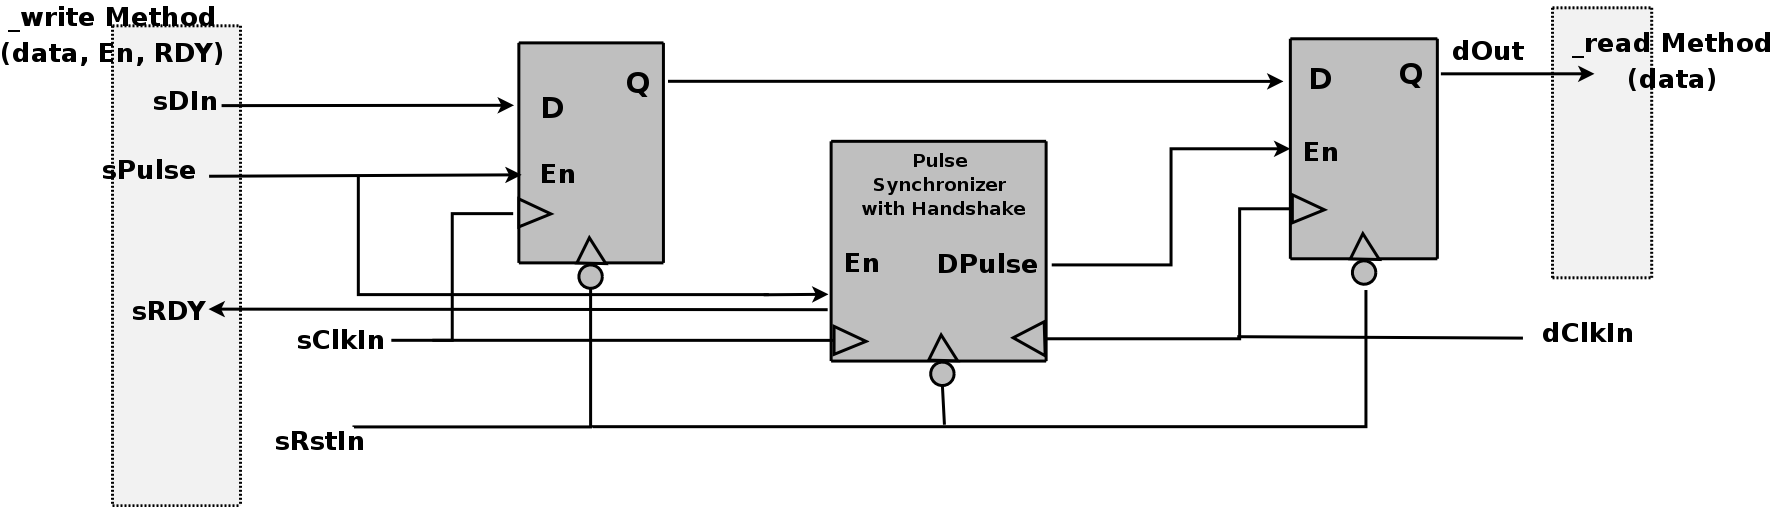
\includegraphics[height = 1.5 in]{LibFig/syncregister}
\caption{Register Synchronization Module (see Figure
\ref{synchandshake} for the pulse synchronizer with handshake)}
\label{syncregister}
\end{center}
\end{figure}

\begin{center}
\begin{tabular}{|p{1.4 in}|p{4.2 in}|}
\hline
&\\
\te{mkSyncReg}&Provides word synchronization across clock domains.  The in and out clocks,
along with the input reset, are explicitly provided.  The default clock
and reset are ignored.   \\
\cline{2-2}
&\begin{libverbatim}
module mkSyncReg #( a_type initValue,
                    Clock sClkIn, Reset sRstIn,
                    Clock dClkIn ) 
                  ( Reg #(a_type) )
   provisos (Bits#(a_type, sa) ) ;
\end{libverbatim}     
\\
\hline
\end{tabular}
\end{center} 

\index[function]{Clocks!mkSyncRegFromCC}
\index{mkSyncRegFromCC@\te{mkSyncRegFromCC} (module)}      
\begin{center}
\begin{tabular}{|p{1.4 in}|p{4.2 in}|}
\hline
&\\
\te{mkSyncRegFromCC}& Provides word synchronization from the current
clock domain.  The input clock and reset are the
current clock and reset.\\
\cline{2-2}
&\begin{libverbatim}
module mkSyncRegFromCC #( a_type initValue, 
                          Clock dClkIn )
                        ( Reg #(a_type) )
   provisos (Bits#(a_type, sa)) ; 
\end{libverbatim}     
\\
\hline
\end{tabular}
\end{center} 

\index[function]{Clocks!mkSyncRegToCC}
\index{mkSyncRegToCC@\te{mkSyncRegToCC} (module)}
\begin{center}
\begin{tabular}{|p{1.4 in}|p{4.2 in}|}
\hline
&\\
\te{mkSyncRegToCC}&Provides word synchronization to the current clock
domain. The
output clock is the current clock. The current reset is ignored.  \\
\cline{2-2}
&\begin{libverbatim}
module mkSyncRegToCC #( a_type initValue,
                        Clock sClkIn, Reset sRstIn )
                      ( Reg #(a_type) )
   provisos (Bits#(a_type, sa)) ;
\end{libverbatim}     
\\
\hline
\end{tabular}
\end{center} 

{\bf Verilog Modules}

The {\BSV} modules correspond to the following {\V}
modules, which are found in the BSC {\V} library, \te{\$BLUESPECDIR/Verilog/}.


\begin{center}
\begin{tabular}{|p {2.8 in}|p{2.8 in}|}
\hline
&\\
BSV Module Name & Verilog Module Name  \\
&\\
\hline
\hline
\te{mkSyncReg}&\te{SyncRegister.v}\\
\te{mkSyncRegFromCC}&\\
\te{mkSyncRegToCC}&\\
\hline
\end{tabular}
\end{center}
%===================================================================
\subsubsection{FIFO Synchronizers}

\index{SyncFIFOIfc@\te{SyncFIFOIfc} (interface)}
\label{syncfifoifc}

{\bf Description}

The \te{SyncFIFO} modules use FIFOs to synchronize data being sent
across clock domains, providing registered
full and empty signals (\te{notFull} and \te{notEmpty}). %  The
% \te{SyncFIFOFull} modules allow the user to choose whether or not the
% full and empty signals are registered.
Additional FIFO synchronizers,
\te{SyncFIFOLevel} and \te{SyncFIFOCount} can be found in the
\te{FIFOLevel} package (Section \ref{FIFOLevel}).  

{\bf Interfaces and Methods}

The \te{SyncFIFOIfc} interface defines an interface similar to the FIFOF
interface, except it does not have a \te{clear} method.

\begin{center}
\begin{tabular}{|p{.5in}|p{.7in}|p{1.8 in}|p{.6in}|p{1.2 in}|}
\hline
\multicolumn{5}{|c|}{\te{SyncFIFOIfc} Interface}\\
\hline
\multicolumn{3}{|c|}{Method}&\multicolumn{2}{|c|}{Arguments}\\
\hline
Name & Type & Description& Name &\multicolumn{1}{|c|}{Description} \\
\hline
\hline 
\te{enq}&\te{Action}&Adds an entry to the FIFO &\te{sendData}&Data
to be added\\
\hline
\te{deq}&\te{Action}&Removes the first entry from the FIFO&&\\
\hline
\te{first}&\te{a\_type}&Returns the first entry&&\\
\hline
\te{notFull}&\te{Bool}&Returns True if there is space and you can
\te{enq} into the FIFO &&\\
\hline
\te{notEmpty}&\te{Bool}&Returns True if there are elements in the FIFO
and you can \te{deq} from the FIFO&&\\
\hline
\end{tabular}
\end{center}

\begin{libverbatim}
     interface SyncFIFOIfc #(type a_type) ;
        method Action enq ( a_type sendData ) ;
        method Action deq () ;
        method a_type first () ; 
        method Bool notFull () ;
        method Bool notEmpty () ;
     endinterface
\end{libverbatim}


{\bf Modules}

\begin{figure}[ht]
\begin{center}
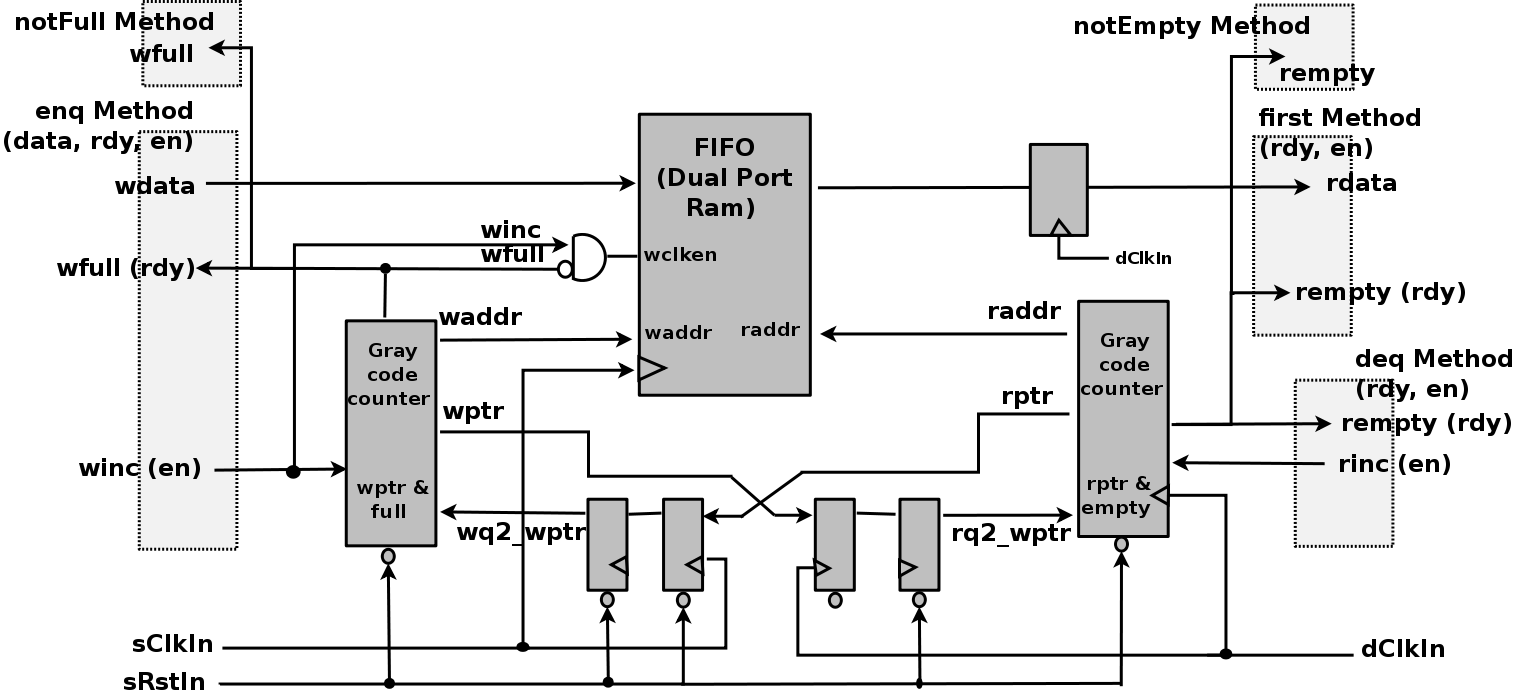
\includegraphics[width  = 5.5 in]{LibFig/syncfifo}
\caption{Synchronization FIFOs}
\label{syncfifo}
\end{center}
\end{figure}

\index[function]{Clocks!mkSyncFIFO}
\index{mkSyncFIFO@\te{mkSyncFIFO} (module)}
The \te{mkSyncFIFO}, \te{mkSyncFIFOFromCC} and \te{mkSyncFIFOToCC} modules
provide FIFOs for sending data across clock domains.  Data items
enqueued on the source side will arrive at the destination side and
remain  there until they are dequeued.  The depth of the FIFO is
specified by the \te{depth} parameter.  The full and empty signals are
registered.  The module \te{mkSyncFIFO1} is a 1 element synchronized FIFO.


\begin{center}
\begin{tabular}{|p{1.4 in}|p{4.2 in}|}
\hline
&\\
\te{mkSyncFIFO}&Provides a FIFO for sending data across clock domains.
 The \te{enq} method is in the source (\te{sClkIn}) domain, while the
 \te{deq}  and
 \te{first} methods are in the destination (\te{dClkIn}) domain.  The in and out clocks,
along with the input reset, are explicitly provided.  The default clock
and reset are ignored. \\
\cline{2-2}
&\begin{libverbatim}
module mkSyncFIFO #( Integer depth,
                     Clock sClkIn, Reset sRstIn,
                     Clock dClkIn )
                   ( SyncFIFOIfc #(a_type) )
   provisos (Bits#(a_type, sa));
\end{libverbatim}     
\\
\hline
\end{tabular}
\end{center} 
      
\index[function]{Clocks!mkSyncFIFOFromCC}
\index{mkSyncFIFOFromCC@\te{mkSyncFIFOFromCC} (module)}
\begin{center}
\begin{tabular}{|p{1.4 in}|p{4.2 in}|}
\hline
&\\
\te{mkSyncFIFOFromCC}&Provides a  FIFO to send data from the
current clock domain into a second clock domain. The input clock and reset are the
current clock and reset.\\
\cline{2-2}
&\begin{libverbatim}
module mkSyncFIFOFromCC #( Integer depth,
                           Clock dClkIn )
                         ( SyncFIFOIfc #(a_type) )
   provisos (Bits#(a_type, sa));
\end{libverbatim}     
\\
\hline
\end{tabular}
\end{center} 

\index[function]{Clocks!mkSyncFIFOToCC}
\index{mkSyncFIFOToCC@\te{mkSyncFIFOToCC} (module)}
\begin{center}
\begin{tabular}{|p{1.4 in}|p{4.2 in}|}
\hline
&\\
\te{mkSyncFIFOToCC}&Provides a  FIFO to send data from a
second clock domain into the current clock domain. The
output clock is the current clock. The current reset is ignored.   \\
\cline{2-2}
&\begin{libverbatim}
module mkSyncFIFOToCC #( Integer depth,
                         Clock sClkIn, Reset sRstIn )
                       ( SyncFIFOIfc #(a_type) )
   provisos (Bits#(a_type, sa));
\end{libverbatim}     
\\
\hline
\end{tabular}
\end{center} 

\index[function]{Clocks!mkSyncFIFO1}
\index{mkSyncFIFO1@\te{mkSyncFIFO1} (module)}

\begin{center}
\begin{tabular}{|p{1.4 in}|p{4.2 in}|}
\hline
&\\
\te{mkSyncFIFO1}&Provides a 1 element FIFO for sending data across
clock domains.  The 1 element module does not have a dedicated output
register and registers for full and empty, as in the depth > 1 module.
This module should be used in clock crossing applications where
complete FIFO handshaking is required, but data throughput or storage
is minimal.   \\
\cline{2-2}
&\begin{libverbatim}
module mkSyncFIFO #( Clock sClkIn, Reset sRstIn,
                     Clock dClkIn )
                   ( SyncFIFOIfc #(a_type) )
   provisos (Bits#(a_type, sa));
\end{libverbatim}     
\\
\hline
\end{tabular}
\end{center} 




%The following syncfifos were deprecated 12/21/10

% The sync FIFOFull modules are a variation of the Sync FIFO which allow
% the user to choose if the empty and full 
% signals are registered.  Registering the signals can give better
% synthesis results, since a comparator is removed from the empty or
% full path.  However, there is an additional cycle of latency
% before the empty or full signal is visible.
% \index[function]{Clocks!mkSyncFIFOFull}
% \index{mkSyncFIFOFull@\te{mkSyncFIFOFull} (module)}
% \begin{center}
% \begin{tabular}{|p{1.4 in}|p{4.2 in}|}
% \hline
% &\\
% \te{mkSyncFIFOFull}&Provides a registered FIFO for sending data across
% clock domains.  The in and out clocks,
% along with the input reset, are explicitly provided.  The default clock
% and reset are ignored. \\
% \cline{2-2}
% &\begin{libverbatim}
% module mkSyncFIFOFull #( Integer depth,  
%                          Bool regEmpty, 
%                          Bool regFull,
%                          Clock sClkIn, Reset sRstIn,
%                          Clock dClkIn )
%                        ( SyncFIFOIfc #(a_type) )
%    provisos (Bits#(a_type, sa));
% \end{libverbatim}     
% \\
% \hline
% \end{tabular}
% \end{center} 

% \index[function]{Clocks!mkSyncFIFOFromCCFull}
% \index{mkSyncFIFOFromCCFull@\te{mkSyncFIFOFromCCFull} (module)}
% \begin{center}
% \begin{tabular}{|p{1.4 in}|p{4.2 in}|}
% \hline
% &\\
% \te{mkSyncFIFOFromCCFull}&Provides a registered FIFO to send data from the
% current clock domain into a second clock domain.  The input clock and reset are the
% current clock and reset. \\
% \cline{2-2}
% &\begin{libverbatim}
% module mkSyncFIFOFromCCFull #( Integer depth, 
%                                Bool regEmpty, 
%                                Bool regFull,
%                                Clock dClkIn )
%                              ( SyncFIFOIfc #(a_type) )
%    provisos (Bits#(a_type, sa));
% \end{libverbatim}     
% \\
% \hline
% \end{tabular}
% \end{center} 

% \index[function]{Clocks!mkSyncFIFOToCCFull}
% \index{mkSyncFIFOToCCFull@\te{mkSyncFIFOToCCFull} (module)}
% \begin{center}
% \begin{tabular}{|p{1.4 in}|p{4.2 in}|}
% \hline
% &\\
% \te{mkSyncFIFOToCCFull}&Provides a registered FIFO to send data from a
% second clock domain into the current clock domain. The
% output clock is the current clock. The current reset is ignored.  \\
% \cline{2-2}
% &\begin{libverbatim}
% module mkSyncFIFOToCCFull #( Integer depth, 
%                              Bool regEmpty, 
%                              Bool regFull,
%                              Clock sClkIn, Reset sRstIn )
%                            ( SyncFIFOIfc #(a_type) )
%    provisos (Bits#(a_type, sa));
% \end{libverbatim}     
% \\
% \hline
% \end{tabular}
% \end{center} 

{\bf Verilog Modules}

The {\BSV} modules correspond to the following {\V}
modules, which are found in the BSC {\V} library, \te{\$BLUESPECDIR/Verilog/}.


\begin{center}
\begin{tabular}{|p {2.8 in}|p{2.8 in}|}
\hline
&\\
BSV Module Name & Verilog Module Name  \\
&\\
\hline
\hline
\te{mkSyncFIFO}&\te{SyncFIFO.v}\\
\te{mkSyncFIFOFromCC}&\\
\te{mkSyncFIFOToCC}&\\
\hline
\te{mkSyncFIFO1}&\te{SyncFIFO1.v}\\
% \te{mkSyncFIFOFull}&\\
% \te{mkSyncFIFOFromCCFull}&\\
% \te{mkSyncFIFOToCCFull}&\\
\hline
\end{tabular}
\end{center}
%====================================================================
\subsubsection{Asynchronous RAMs}
\index{DualPortRamIfc@\te{DualPortRamIfc} (interface)}
\index{mkDualRam@\te{mkDualRam} (module)}
\index[function]{Clocks!mkDualRam}

{\bf Description}

An asynchronous RAM provides a domain crossing by having its read and
write methods in separate clock domains.

{\bf Interfaces and Methods}

\begin{center}
\begin{tabular}{|p{.5in}|p{.5in}|p{1.6 in}|p{.5in}|p{1.7 in}|}
\hline
\multicolumn{5}{|c|}{\te{DualPortRamIfc} Interface}\\
\hline
\multicolumn{3}{|c|}{Method}&\multicolumn{2}{|c|}{Arguments}\\
\hline
Name & Type & Description& Name &\multicolumn{1}{|c|}{Description} \\
\hline
\hline 
\te{write}&\te{Action}&Writes data to a an address in a
RAM&\te{wr\_addr}&Address of datatype \te{addr\_t}\\
& &&\te{din}&Data of datatype \te{data\_t}\\
\hline
\te{read}&\te{data\_d}&Reads the data from the
RAM&\te{rd\_addr}&Address to be read from\\
\hline
\end{tabular}
\end{center}

\begin{libverbatim}
     interface DualPortRamIfc #(type addr_t, type data_t);
        method Action      write( addr_t wr_addr, data_t  din );
        method data_t      read ( addr_t rd_addr);
     endinterface: DualPortRamIfc
\end{libverbatim}


\begin{figure}[ht]
\begin{center}
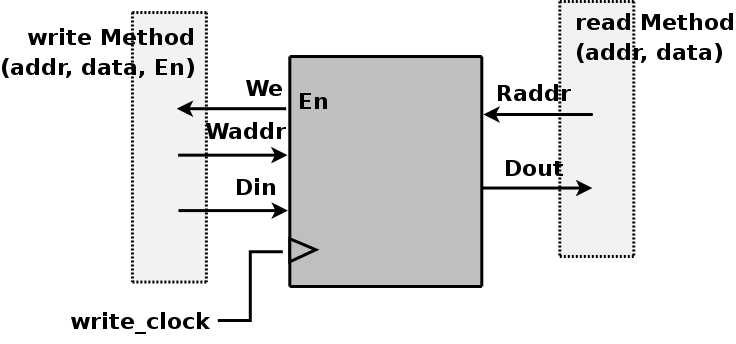
\includegraphics[height = 1.2 in]{LibFig/dualram}
\caption{Ansynchronous RAM}
\label{dualram}
\end{center}
\end{figure}


\begin{center}
\begin{tabular}{|p{1.4 in}|p{4.2 in}|}
\hline
&\\
\te{mkDualRam}&Provides an asynchronous RAM for  when the read and the
write  methods are in separate
clock domains.  The write method is clocked by the default clock, the
read method is not clocked.\\
\cline{2-2}
&\begin{libverbatim}
module mkDualRam( DualPortRamIfc #(addr_t, data_t) )
   provisos ( Bits#(addr_t, sa),
              Bits#(data_t, da) ) ;
\end{libverbatim}     
\\
\hline
\end{tabular}
\end{center} 

{\bf Verilog Modules}

The {\BSV} modules correspond to the following {\V}
modules, which are found in the BSC {\V} library, \te{\$BLUESPECDIR/Verilog/}.


\begin{center}
\begin{tabular}{|p {2.8 in}|p{2.8 in}|}
\hline
&\\
BSV Module Name & Verilog Module Name  \\
&\\
\hline
\hline
\te{mkDualRam}&\te{DualPortRam.v}\\
\hline
\end{tabular}
\end{center}
%=======================================================================
\subsubsection{Null Crossing Primitives}
%\index{ReadOnly@\te{ReadOnly} (interface)}

{\bf Description}

In these primitives, no synchronization is actually done.    It is up to
the  designer to verify that it is safe for the signal to be used in
the other domain. The \te{mkNullCrossingWire} is a wire synchronizer.
The \te{mkNullCrossingReg} modules are equivalent to a register
(\te{mkReg}, \te{mkRegA}, or \te{mkRegU} depending on the module)
followed by a \te{mkNullCrossingWire}.  

The older \te{mkNullCrossing} primitive is deprecated.

{\bf Interfaces} 

The \te{mkNullCrossingWire} module, shown in Figure \ref{syncwire},
provides the \te{ReadOnly} interface which is defined in the Prelude
library \ref{readonly}.

The \te{mkNullCrossingReg} modules provide the \te{CrossingReg}
interface.

{\bf Interfaces and Methods}

\begin{center}
\begin{tabular}{|p{.5in}|p{.5in}|p{1.6 in}|p{.5in}|p{1.7 in}|}
\hline
\multicolumn{5}{|c|}{\te{CrossingReg} Interface}\\
\hline
\multicolumn{3}{|c|}{Method}&\multicolumn{2}{|c|}{Arguments}\\
\hline
Name & Type & Description& Name &\multicolumn{1}{|c|}{Description} \\
\hline
\hline 
\te{\_write}&Action&Writes a value \te{datain}&\te{datain}&Data to be
written.\\
\hline
\te{\_read}&\te{a\_type}&Returns the value of the register in the
source clock domain&&\\
\hline
\te{crossed}&\te{a\_type}&Returns the value of the register in the
destination clock domain&&\\
\hline
\end{tabular}
\end{center}

\begin{libverbatim}
interface CrossingReg #( type a_type ) ;
   method Action _write(a datain) ;
   method a_type _read() ;
   method a_type crossed() ;
endinterface
\end{libverbatim}



{\bf Modules}

\begin{figure}[htb]
\begin{center}
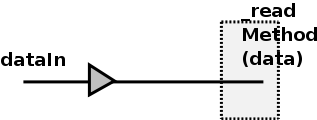
\includegraphics[height = .8 in]{LibFig/syncwire}
\caption{Wire synchronizer}
\label{syncwire}
\end{center}
\end{figure}


\index[function]{Clocks!mkNullCrossingWire}
\index{mkNullCrossingWire@\te{mkNullCrossingWire} (module)}
\begin{center}
\begin{tabular}{|p{1.4 in}|p{4.2 in}|}
\hline
&\\
\te{mkNullCrossingWire}&Defines a synchronizer that contains only a wire.
It is left up to the designer to ensure the clock crossing is safe.\\
\cline{2-2}
&\begin{libverbatim}
module mkNullCrossingWire #( Clock dClk, a_type dataIn )
                           ( ReadOnly#(a_type) )
   provisos (Bits#(a_type, sa)) ;
\end{libverbatim}     
\\
\hline
\end{tabular}
\end{center} 

\begin{figure}[htb]
\begin{center}
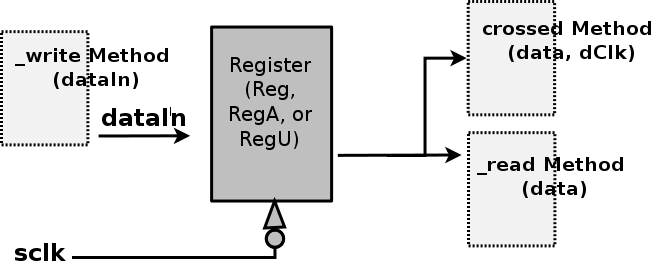
\includegraphics[height = 1.2 in]{LibFig/nullcrossingreg}
\caption{Register with wire synchronizer}
\label{nullcrossingreg}
\end{center}
\end{figure}

\index[function]{Clocks!mkNullCrossingReg}
\index{mkNullCrossingReg@\te{mkNullCrossingReg} (module)}
\begin{center}
\begin{tabular}{|p{1.4 in}|p{4.2 in}|}
\hline
&\\
\te{mkNullCrossingReg}&Defines a synchronizer that contains a register
with a synchronous reset value, 
followed by a wire synchronizer.
It is left up to the designer to ensure the clock crossing is safe.\\
\cline{2-2}
&\begin{libverbatim}
module mkNullCrossingReg( Clock dClk, a_type resetval, 
                          CrossingReg#(a_type) ifc )
   provisos (Bits#(a_type, sz_a)) ;
\end{libverbatim}     
\\
\hline
\end{tabular}
\end{center} 


\index[function]{Clocks!mkNullCrossingRegA}
\index{mkNullCrossingRegA@\te{mkNullCrossingRegA} (module)}
\begin{center}
\begin{tabular}{|p{1.4 in}|p{4.2 in}|}
\hline
&\\
\te{mkNullCrossingRegA}&Defines a synchronizer that contains a register
with a given reset value where reset is asynchronous, followed by a wire synchronizer.
It is left up to the designer to ensure the clock crossing is safe.\\
\cline{2-2}
&\begin{libverbatim}
module mkNullCrossingRegA( Clock dClk, a_type resetval, 
                          CrossingReg#(a_type) ifc )
   provisos (Bits#(a_type, sz_a)) ;
\end{libverbatim}     
\\
\hline
\end{tabular}
\end{center} 

\index[function]{Clocks!mkNullCrossingRegU}
\index{mkNullCrossingRegU@\te{mkNullCrossingRegU} (module)}
\begin{center}
\begin{tabular}{|p{1.4 in}|p{4.2 in}|}
\hline
&\\
\te{mkNullCrossingRegU}&Defines a synchronizer that contains a register
without a reset, followed by a wire synchronizer.
It is left up to the designer to ensure the clock crossing is safe.\\
\cline{2-2}
&\begin{libverbatim}
module mkNullCrossingRegU( Clock dClk, 
                           CrossingReg#(a_type) ifc )
   provisos (Bits#(a_type, sz_a)) ;
\end{libverbatim}     
\\
\hline
\end{tabular}
\end{center} 


{\bf Example: instantiating a null synchronizer }
\begin{libverbatim}
   // domain2sig is domain1sig synchronized to clk0 with just a wire.
   ReadOnly#(Bit#(2)) domain2sig <- mkNullCrossingWire (clk0, domain1sig);
\end{libverbatim}

Note: no synchronization is actually done.  This is purely a way to
tell BSC that it is safe to use the signal in the other
domain.  It is the responsibility of the designer to verify that this
is correct.

There are some restrictions on the use of a \te{mkNullCrossingWire}.
The expression used as the data argument must not have an implicit
condition, and there cannot be another rule which is required to 
schedule before any method called in the expression.

\te{mkNullCrossingWire}s may not be used in sequence to pass a signal
across multiple clock boundaries without synchronization.  Once a
signal has been crossed from one domain to a second domain without
synchronization, it cannot be subsequently passed unsynchronized to a
third domain (or back to the first domain).

{\bf Verilog Modules}

The {\BSV} modules correspond to the following {\V}
modules, which are found in the BSC {\V} library, \te{\$BLUESPECDIR/Verilog/}.

\begin{center}
\begin{tabular}{|p {2.8 in}|p{2.8 in}|}
\hline
&\\
BSV Module Name & Verilog Module Name  \\
&\\
\hline
\hline
\te{mkNullCrossingWire}&\te{BypassWire.v}\\
\hline
\end{tabular}
\end{center}
%===================================================================
% \subsubsection{Specialized Crossing Primitives}
% \label{crossing-prim}   
% \index{mkSynRegToSlow@\te{mkSyncRegToSlow} (module)}
% \index{mkSyncRegToFast@\te{mkSyncRegToFast} (module)}
% \index{mkSyncFIFOToSlow@\te{mkSyncFIFOToSlow} (module)}
% \index{mkSyncFIFOToFast@\te{mkSyncFIFOToFast} (module)}
% \index[function]{Clocks!mkSyncRegToSlow}
% \index[function]{Clocks!mkSyncRegToFast}
% \index[function]{Clocks!mkSyncFIFOToSlow}
% \index[function]{Clocks!mkSyncFIFOToFast}
% {\bf Description}




% The {\tt mkSyncRegToSlow} and {\tt mkSyncRegToFast} are specialized crossing primitives
% which can be used to transport data when clock edges are aligned,
% between the domains. The divided clocks and the appropriate
% interface needed for the module would typically be
% generated using the {\tt mkClockDivider} module (Section \ref{sec-clockdivider}).

% The crossing primitive is implemented via a single register,
% clocked by the slower (divided) clock.  For a fast  to slow crossing, the
% register  is only writable when the {\tt
% clockReady} bit of the divider interface is asserted.  This is an
% implicit  condition of the write method 
% module which prevents erroneous writes.  For a slow to fast
% crossing both the read and write methods are always available. 

% {\bf Modules}

% \begin{figure}[ht]
% \begin{center}
% 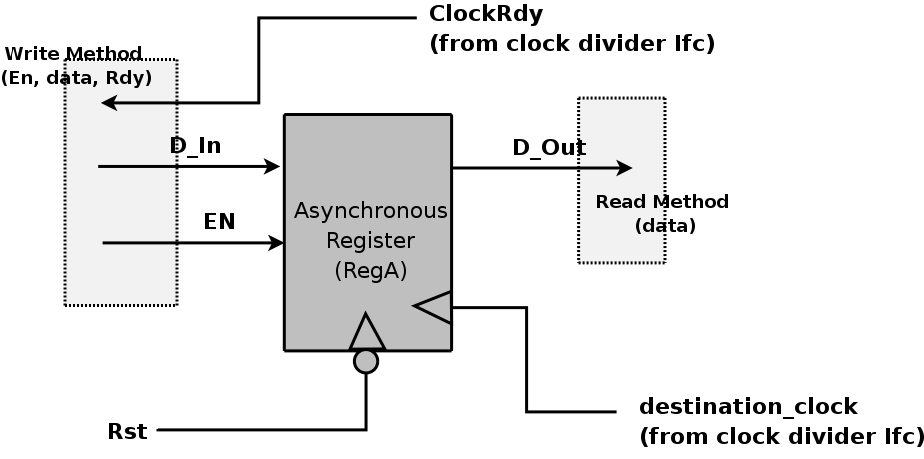
\includegraphics[height = 1.5 in]{LibFig/SyncRegSlow}
% \caption{Fast to Slow Crossing}
% \label{syncregslow}
% \end{center}
% \end{figure}


% \begin{center}
% \begin{tabular}{|p{1.4 in}|p{4.2 in}|}
% \hline
% &\\
% \te{mkSyncRegToSlow}&Provides a register to transport data when the
% clock edges are aligned between domains.  This module moves data from a
% fast to a slow domain.  The register is only writable when the {\tt
% clockReady} bit of the divider is asserted. \\
% \cline{2-2}
% &\begin{libverbatim}
% module mkSyncRegToSlow #( a_type initValue,
%                           ClockDividerIfc divider,
%                           Reset slowRstIn )
%                         ( Reg #(a_type) ) 
%    provisos (Bits#(a_type, sa)) ;
% \end{libverbatim}     
% \\
% \hline
% \end{tabular}
% \end{center} 
   
% \begin{figure}[ht]
% \begin{center}
% 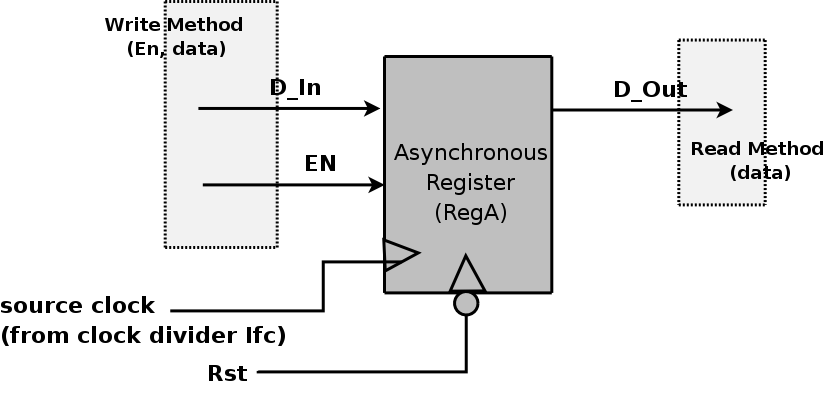
\includegraphics[height = 1.5 in]{LibFig/SyncRegtoFast}
% \caption{Slow to Fast Crossing}
% \label{syncregfast}
% \end{center}
% \end{figure}



% \begin{center}
% \begin{tabular}{|p{1.4 in}|p{4.2 in}|}
% \hline
% &\\
% \te{mkSyncRegToFast}&Provides a register to transport data when the
% clock edges are aligned between domains.  This module moves data from a
% slow to a fast domain.  The read and write methods are always available.  \\
% \cline{2-2}
% &\begin{libverbatim}
% module mkSyncRegToFast #( a_type initValue,
%                           ClockDividerIfc divider,
%                           Reset slowRstIn )
%                         ( Reg #(a_type) ) 
%    provisos (Bits#(a_type, sa)) ;
% \end{libverbatim}     
% \\
% \hline
% \end{tabular}
% \end{center} 
   
% The {\tt mkSyncFIFOToSlow} and {\tt mkSyncFIFOToFast} modules are  specialized crossing
% primitives which can be used to transport data when clock edges are
% aligned, between a fast clock domain and a slower clock domain. 
%  The derived clock and the
% \te{ClkNextRdy} signal would typically be
% generated using the {\tt mkClockDivider} module.  The synchronous
% FIFOs are clocked by the slower (divided) clock.  The \te{SyncFIFOIfc} is detailed
% in Section \ref{syncfifoifc}.

% \begin{figure}[ht]
% \begin{center}
% 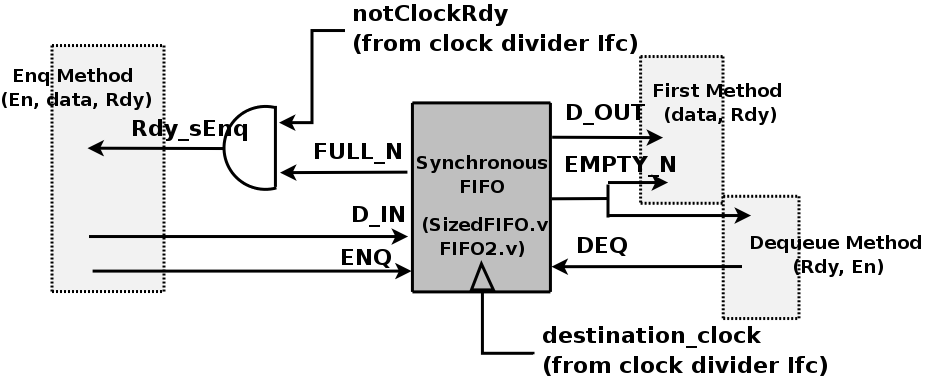
\includegraphics[height = 1.5 in]{LibFig/syncfifotoslow}
% \caption{Aligned clocks with FIFO - to slower domain}
% \label{fifotoslow}
% \end{center}
% \end{figure}


% \begin{center}
% \begin{tabular}{|p{1.4 in}|p{4.2 in}|}
% \hline
% &\\
% \te{mkSyncFIFOToSlow}&Provides a FIFO with specified depth to transport data from a fast clock domain
% to a slower clock domain when clock edges are aligned. The crossing primitive is implemented via a FIFO with the
% specified depth
% clocked by \te{dClkIn}. The FIFO is
% enqueued only when the {\tt syncBit} is asserted and the FIFO is not full. \\
% \cline{2-2}
% &\begin{libverbatim}
% module mkSyncFIFOToSlow #( Integer depth,
%                            ClockDividerIfc divider,
%                            Reset slowRstIn )
%                          ( SyncFIFOIfc #(a_type) ) 
%    provisos (Bits#(a_type, sa)) ;
% \end{libverbatim}     
% \\
% \hline
% \end{tabular}
% \end{center} 
      
% \begin{figure}[ht]
% \begin{center}
% 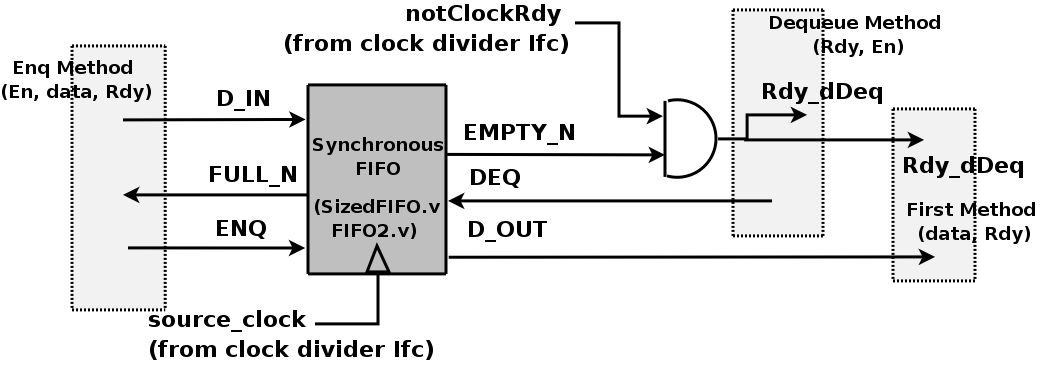
\includegraphics[height = 1.5 in]{LibFig/syncfifotofast}
% \caption{Aligned clocks with FIFO - to faster domain}
% \label{fifotofast}
% \end{center}
% \end{figure}


% \begin{center}
% \begin{tabular}{|p{1.4 in}|p{4.2 in}|}
% \hline
% &\\
% \te{mkSyncFIFOToFast}&Provides a FIFO with specified depth to
% transport data  from a slower clock domain
% to a faster clock domain when clock edges are aligned.  The crossing
% primitive  is implemented via a FIFO with the specified depth
% clocked by sClkIn (the source clock is the slower clock).
%  The FIFO is
% dequeued only when the {\tt syncBit} is asserted and the FIFO is not empty.   \\
% \cline{2-2}
% &\begin{libverbatim}
% module mkSyncFIFOToFast #( Integer depth,
%                            ClockDividerIfc divider,
%                            Reset slowRstIn )
%                          ( SyncFIFOIfc #(a_type) ) 
%    provisos (Bits#(a_type, sa)) ;
% \end{libverbatim}     
% \\
% \hline
% \end{tabular}
% \end{center} 

% {\bf Verilog Modules}

% The {\BSV} modules correspond to the following {\V}
% modules, which are found in the BSC {\V} library, \te{\$BLUESPECDIR/Verilog/}.

% \begin{center}
% \begin{tabular}{|p {2.8 in}|p{2.8 in}|}
% \hline
% &\\
% BSV Module Name & Verilog Module Name  \\
% &\\
% \hline
% \hline
% \te{mkSyncRegToSlow}&\te{RegA.v}\\
% \te{mkSyncRegToFast}&\\
% \hline
% \te{mkSyncFIFOToSlow}& \te{FIFO2.v}\\
% \te{mkSyncFIFOToFast}&\te{SizedFIFO.v}\\
% \hline
% \end{tabular}
% \end{center}
%===========================================================
\subsubsection{Reset Synchronization and Generation}



{\bf Description}

This section describes the interfaces and modules used to synchronize
reset signals from one clock domain to another and to 
create  reset signals.   Reset generation converts a Boolean type to a
Reset type, where the reset is associated with the default or
\te{clocked\_by} clock domain.


{\bf Interfaces and Methods}
\index{MakeResetIfc@\te{MakeResetIfc} (interface)}
\index{MuxRstIfc@\te{MuxRstIfc} (interface)}

The \te{MakeResetIfc} interface is provided by the reset generators
\te{mkReset} and \te{mkResetSync}.


\begin{center}
\begin{tabular}{|p{1 in}|p{1 in}|p{3 in}|}
\hline
\multicolumn{3}{|c|}{\te{MakeResetIfc} Interface}\\
\hline
\multicolumn{3}{|c|}{Method}\\
\hline
Name & Type & Description\\
\hline
\hline 
\te{assertReset}&\te{Action}&Method used to assert the reset\\
\hline
\te{isAsserted}&\te{Bool}&Indicates whether the reset is asserted\\
\hline
\te{new\_rst}&\te{Reset}&Generated output reset\\
\hline
\end{tabular}
\end{center}


\begin{libverbatim}
     interface MakeResetIfc;
        method Action assertReset();
        method Bool isAsserted();
        interface Reset new_rst;
     endinterface
\end{libverbatim}


The interface \te{MuxRstIfc} is provided by the \te{mkResetMux} module.

\begin{center}
\begin{tabular}{|p{.7in}|p{.7in}|p{1.5 in}|p{.4in}|p{1.5 in}|}
\hline
\multicolumn{5}{|c|}{\te{MuxRstIfc} Interface}\\
\hline
\multicolumn{3}{|c|}{Method}&\multicolumn{2}{|c|}{Arguments}\\
\hline
Name & Type & Description& Name &\multicolumn{1}{|c|}{Description} \\
\hline
\hline 
\te{select}&\te{Action}&Method used to select the reset based on the
Boolean value \te{ab}  &\te{ab}   &Value determines which input reset
to select\\
\hline
\te{reset\_out}&\te{Reset}&Generated output reset &&\\
\hline
\end{tabular}
\end{center}


\begin{libverbatim}
     interface MuxRstIfc;
        method Action select ( Bool ab );
        interface Reset reset_out;
     endinterface
\end{libverbatim}

{\bf Modules}
\index{mkSyncReset@\te{mkSyncReset} (module)}
\index{mkSyncResetFromCR@\te{mkSyncResetFromCR} (module)}
\index{mkAsyncReset@\te{mkAsyncReset} (module)}
\index{mkAsyncResetFromCR@\te{mkAsyncResetFromCR} (module)}
\index[function]{Clocks!mkSyncReset}
\index[function]{Clocks!mkSyncResetFromCR}
\index[function]{Clocks!mkAsyncReset}
\index[function]{Clocks!mkAsyncResetFromCR}


\paragraph{Reset Synchronization}

To synchronize resets from one clock domain to another, both
synchronous and asynchronous
modules are provided. 
The  {\tt stages} argument is the number of full clock cycles the
output reset is held for after the input reset is deasserted.  This
is shown as the number of flops in figures \ref{syncreseta} and \ref{syncreset}.
Specifying a 0 for the \te{stages} argument results in the creation of
a simple wire between \te{sRst} and \te{dRstOut}.

\begin{figure}[ht]
\begin{center}
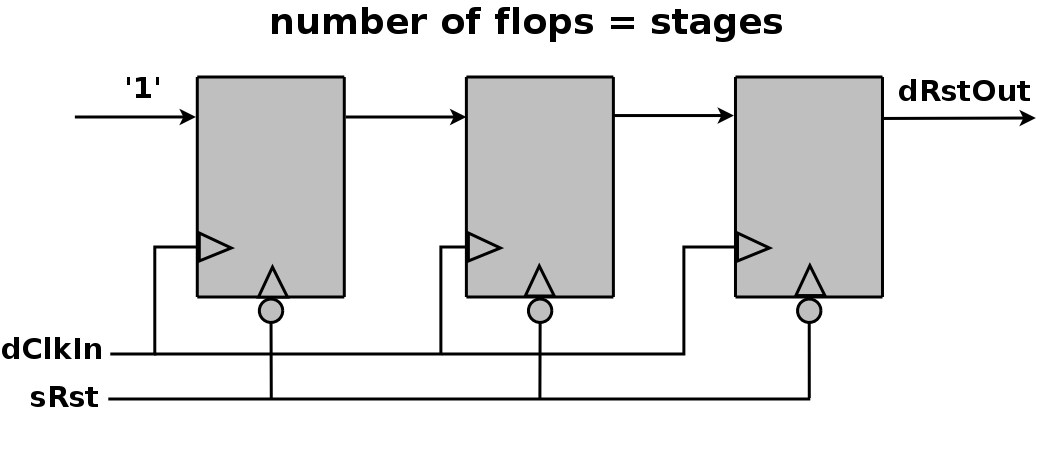
\includegraphics[height = 1.3 in]{LibFig/syncreseta}
\caption{Module for asynchronous resets}
\label{syncreseta}
\end{center}
\end{figure}


\begin{center}
\begin{tabular}{|p{1.4 in}|p{4.2 in}|}
\hline
&\\
\te{mkAsyncReset}&Provides synchronization of a source reset (\te{sRst})
to the destination  domain.  The  output reset occurs
immediately once the source reset is asserted.\\
\cline{2-2}
&\begin{libverbatim}
module mkAsyncReset #( Integer stages,
                       Reset sRst, 
                       Clock dClkIn ) 
                     ( Reset ) ;
\end{libverbatim}     
\\
\hline
\end{tabular}
\end{center} 

\begin{center}
\begin{tabular}{|p{1.4 in}|p{4.2 in}|}
\hline
&\\
\te{mkAsyncResetFromCR}&Provides synchronization of the
current reset to the destination domain.  There is no source reset \te{sRst}
argument because it is taken from the current reset.  The output reset
occurs immediately once the current reset is asserted.\\
\cline{2-2}
&\begin{libverbatim}
module mkAsyncResetFromCR #( Integer stages, 
                             Clock dClkIn )
                           ( Reset ) ;
\end{libverbatim}     
\\
\hline
\end{tabular}
\end{center} 


The less common {\tt mkSyncReset} modules are provided for
convenience, but these modules {\em require} that {\tt sRst} be held
during a positive edge of {\tt dClkIn} for the reset assertion to
be detected.  
Both \te{mkSyncReset} and \te{mkSyncResetFromCR} use the model in figure \ref{syncreset}.

\begin{figure}[ht]
\begin{center}
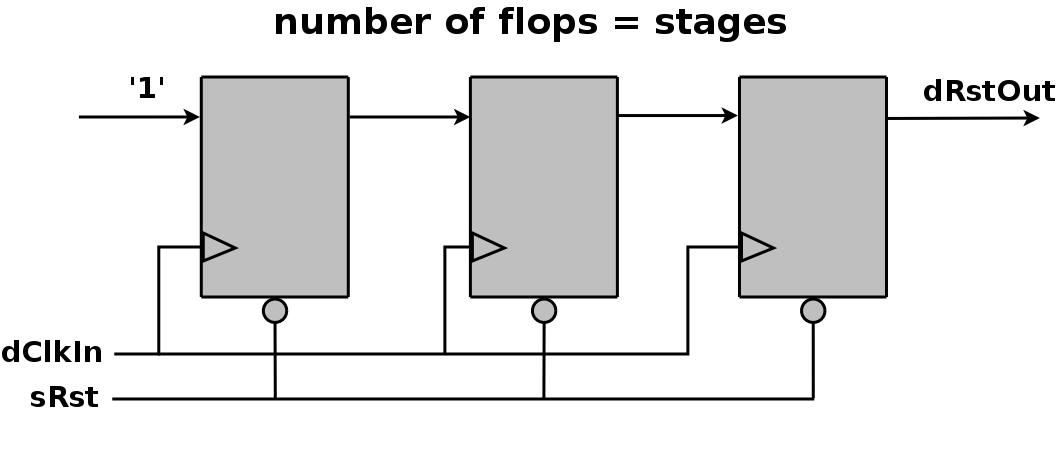
\includegraphics[height = 1.3 in]{LibFig/syncreset}
\caption{Module for synchronous resets}
\label{syncreset}
\end{center}
\end{figure}


\begin{center}
\begin{tabular}{|p{1.4 in}|p{4.2 in}|}
\hline
&\\
\te{mkSyncReset}& Provides synchronization of a source reset (\te{sRst})
to the destination  domain. 
The reset is asserted at the next rising edge of the clock.\\
\cline{2-2}
&\begin{libverbatim}
module mkSyncReset #( Integer stages 
                      Reset sRst, 
                      Clock dClkIn )
                    ( Reset ) ;
 
\end{libverbatim}     
\\
\hline
\end{tabular}
\end{center} 


\begin{center}
\begin{tabular}{|p{1.4 in}|p{4.2 in}|}
\hline
&\\
\te{mkSyncResetFromCR}&Provides synchronization of the
current reset to the destination domain.
The reset is asserted
at  the next rising edge of the clock.\\
\cline{2-2}
&\begin{libverbatim}
module mkSyncResetFromCR #( Integer stages 
                            Clock dClkIn ) 
                          ( Reset ) ;
\end{libverbatim}     
\\
\hline
\end{tabular}
\end{center} 






{\bf Example: instantiating a reset synchronizer }
\begin{libverbatim}
   // 2 is the number of stages
   Reset rstn2 <- mkAsyncResetFromCR (2, clk0);

   // if stages = 0, the default reset is used directly
   Reset rstn0 <- mkAsyncResetFromCR (0, clk0);
\end{libverbatim}

\paragraph{Reset Generation}

Two modules are provided for reset generation, {\tt  mkReset} and {\tt
mkResetSync}, where each module has one parameter, {\tt stages}.
The {\tt stages}  parameter is the number of full clock 
cycles the output reset is held after the \te{inRst}, as seen in
figure   \ref{makereseta},  is
deasserted.  Specifying a 0 for the {\tt stages} parameter results
in the creation of a simple wire between the input register and the
output reset.
 That is, the reset is asserted immediately and not held
after the input reset is deasserted.  It becomes the designer's
responsibility to ensure that the input reset is asserted for
sufficient time to allow the design to reset properly. 
The reset is controlled using the \te{assertReset} method of the
\te{MakeResetIfc} interface.
   
The difference between {\tt mkReset} and {\tt mkResetSync}
is that for the former, the assertion of reset is immediate, while
the later asserts reset at the next rising edge of the clock.
Note that use of 
\te{mkResetSync} is less common, since the reset requires clock edges
to take effect; failure to assert reset for a clock edge will 
result in a reset not being seen at the output reset.

\index{mkReset@\te{mkReset} (module)}
\index{mkResetSync@\te{mkResetSync} (module)}
\index{mkInitialReset@\te{mkInitialReset} (module)}
\index[function]{Clocks!mkReset}
\index[function]{Clocks!mkResetSync}
\index[function]{Clocks!mkInitialReset}


\begin{figure}[ht]
\begin{center}
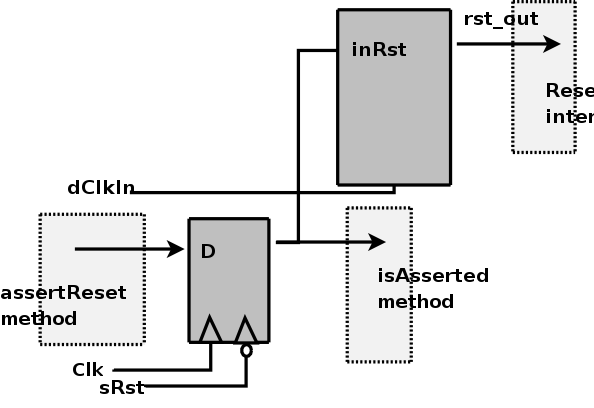
\includegraphics[height = 1.8 in]{LibFig/Makereseta}
\caption{Module for generating resets}
\label{makereseta}
\end{center}
\end{figure}


\begin{center}
\begin{tabular}{|p{1.4 in}|p{4.2 in}|}
\hline
&\\
\te{mkReset}&Provides conversion of a Boolean type to a Reset type,
where the reset is associated with  \te{dClkIn}.
This module uses the  model in figure \ref{makereseta}.
\te{startInRst} indicates the reset value of the register.  
If \te{startInRst} is True, the reset value of the register is 0, which
means the output reset will be asserted whenever the currentReset
(\te{sRst}) is asserted.  \te{rst\_out}  will remain asserted for the number of
clock cycles given by the stages parameter after \te{sRst} is
deasserted.  If \te{startInRst} is False, the output reset will not be
asserted when \te{sRst} is asserted, but only when the
\te{assert\_reset} method is invoked.  At the start of simulation
\te{rst\_out} will only be asserted if \te{startinRst} is True and
\te{sRst} is initially asserted.  \\
\cline{2-2}
&\begin{libverbatim}
module mkReset #( Integer stages,
                  Bool startInRst, 
                  Clock dClkIn )
                ( MakeResetIfc ) ;
\end{libverbatim}     
\\
\hline
\end{tabular}
\end{center} 


   
\begin{center}
\begin{tabular}{|p{1.4 in}|p{4.2 in}|}
\hline
&\\
\te{mkResetSync}& Provides conversion of a Boolean type to a Reset type,
where the reset is associated with  \te{dClkIn}
and the assertion of reset is at the next rising edge of the
clock. This module  uses the  model in figure
\ref{makereseta}.
\te{startInRst} indicates the reset value of the register.  
If \te{startInRst} is True, the reset value of the register is 0, which
means the output reset will be asserted whenever the currentReset
(\te{sRst}) is asserted.  \te{rst\_out}  will remain asserted for the number of
clock cycles given by the stages parameter after \te{sRst} is
deasserted.  If \te{startInRst} is False, the output reset will not be
asserted when \te{sRst} is asserted, but only when the
\te{assert\_reset} method is invoked.  At the start of simulation
\te{rst\_out} will only be asserted if \te{startinRst} is True and
\te{sRst} is initially asserted.  \\
\cline{2-2}
&\begin{libverbatim}
module mkResetSync #( Integer stages,
                      Bool startInRst,
                      Clock dClkIn )
                    ( MakeResetIfc ) ;
\end{libverbatim}     
\\
\hline
\end{tabular}
\end{center} 


\index[function]{Clocks!mkResetMux}
\index{mkResetMux@\te{mkResetMux} (module)}   
  A reset multiplexor {\tt mkResetMux}, as seen in figure
 \ref{resetmux}, 
 creates one reset signal by selecting between two existing reset
signals.  

\begin{figure}[ht]
\begin{center}
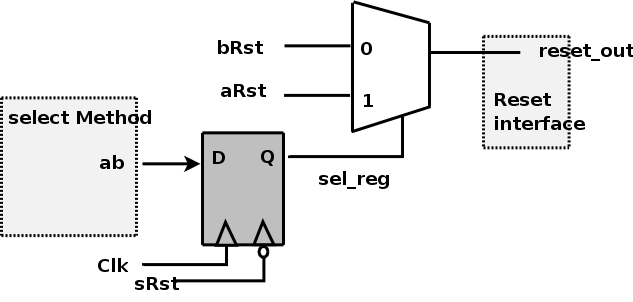
\includegraphics[height=1.4 in]{LibFig/resetmux}
\caption{Reset Multiplexor}
\label{resetmux}
\end{center}
\end{figure}


\begin{center}
\begin{tabular}{|p{1.4 in}|p{4.2 in}|}
\hline
&\\
\te{mkResetMux}& Multiplexor which selects between two input resets,
\te{aRst} and \te{bRst}, to create a single output
reset \te{rst\_out}.  The reset is selected through a Boolean value
provided to the \te{select} method 
where True selects \te{aRst}.\\
\cline{2-2}
&\begin{libverbatim}
module mkResetMux #( Reset aRst, Reset bRst )
                   ( MuxRstIfc rst_out ) ;
\end{libverbatim}     
\\
\hline
\end{tabular}
\end{center} 


For testbenches, in which an absolute clock is being created,
it is helpful to generate a reset for that clock.
The module {\tt mkInitialReset} is available for this purpose.  It
generates a reset which is asserted at the start of simulation.  
The reset is
asserted for  the  number of cycles
specified by  the parameter \te{cycles},  counting the start of time
as 1 cycle. Therefore, a \te{cycles} value of 1 will cause the reset to
turn off at the first clock tick.  
This module is not  synthesizable.   

\begin{center}
\begin{tabular}{|p{1.4 in}|p{4.2 in}|}
\hline
&\\
\te{mkInitialReset}&Generates a reset for \te{cycles} cycles, where
the  \te{cycles} parameter  must be
greater  than zero.  The \te{clocked\_by} clause indicates the clock
the reset is associated with.  This module is not synthesizable.  \\
\cline{2-2}
&\begin{libverbatim}
module mkInitialReset #( Integer cycles )
                       ( Reset ) ;
\end{libverbatim}     
\\
\hline
\end{tabular}
\end{center} 

Example:
\begin{verbatim}
    Clock c <- mkAbsoluteClock (10, 5);
    // a reset associated with clock c:
    Reset r <- mkInitialReset (2, clocked_by c);
\end{verbatim}

\index{mkResetEither@\te{mkResetEither} (module)}
\index[function]{Clocks!mkResetEither}
When two reset signals need to be combined so that some logic can be
reset when either input reset is asserted, the \te{mkResetEither}
module can be used.


\begin{figure}[ht]
\begin{center}
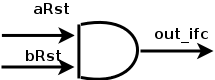
\includegraphics[height=.5 in]{LibFig/resetEither}
\caption{Reset Either}
\label{reseteither}
\end{center}
\end{figure}



\begin{center}
\begin{tabular}{|p{1.4 in}|p{4.2 in}|}
\hline
&\\
\te{mkResetEither}&Generates a reset which is asserted whenever either
input reset is asserted. \\
\cline{2-2}
&\begin{libverbatim}
module mkResetEither ( Reset aRst,
                       Reset bRst)
                     ( Reset out_ifc );
\end{libverbatim}
\\
\hline
\end{tabular}
\end{center} 

Example:
\begin{verbatim}
    Reset r <- mkResetEither(rst1, rst2);
\end{verbatim}

\index{mkResetInverter@\te{mkResetInverter} (module)}
\index[function]{Clocks!mkResetInverter}

\begin{center}
\begin{tabular}{|p{1.4 in}|p{4.2 in}|}
\hline
&\\
\te{mkResetInverter}&Generates an inverted Reset.\\
\cline{2-2}
&\begin{libverbatim}
module mkResetInverter#(Reset in)
                       (Reset);
\end{libverbatim}
\\
\hline
\end{tabular}
\end{center} 

\index{isResetAsserted@\te{isResetAsserted} (module)}
\index[function]{Clocks!isResetAsserted}

\begin{center}
\begin{tabular}{|p{1.4 in}|p{4.2 in}|}
\hline
&\\
\te{isResetAsserted}&Tests whether a Reset is asserted, providing a
Boolean value in the clock domain associated with the Reset.  \\
\cline{2-2}
&\begin{libverbatim}
module isResetAsserted( ReadOnly#(Bool) ifc ) ;
\end{libverbatim}
\\
\hline
\end{tabular}
\end{center} 



{\bf Verilog Modules}

The {\BSV} modules correspond to the following {\V}
modules, which are found in the BSC {\V} library, \te{\$BLUESPECDIR/Verilog/}.

\begin{center}
\begin{tabular}{|p {1.8 in}|p{1.8 in} |p{1.8in}|}
\hline
&&\\
BSV Module Name &Verilog Module Name&Comments  \\
&&\\
\hline
\hline
\te{mkASyncReset}&\te{SyncReset0.v}& when stages==0\\
\cline{2-3}
\te{mkASyncResetFromCR}&\te{SyncResetA.v}&\\
\hline
\te{mkSyncReset}&\te{SyncReset0.v}& when stages==0\\\cline{2-3}
\te{mkSyncResetFromCR}&\te{SyncReset.v}&\\
\hline
\te{mkReset}&\te{MakeReset0.v}&when stages==0\\\cline{2-3}
& \te{MakeResetA.v}&instantiates \te{SyncResetA} \\
\hline
\te{mkResetSync}&\te{MakeReset0.v}&when stages==0\\\cline{2-3}
&\te{MakeReset.v}&instantiates \te{SyncReset} \\
\hline
\te{mkResetMux}&\te{ResetMux.v}&\\
\hline
\te{mkResetEither}&\te{ResetEither.v}&\\
\hline
\te{mkResetInverter}&\te{ResetInverter.v}&\\
\hline
\te{isResetAsserted}&\te{ResetToBool.v}&\\
\hline
\end{tabular}
\end{center}













